% =====================================================================
% Trabajo Dirigido — UFPS — Ingeniería de Sistemas
% Propuesta de analítica predictiva de datos abiertos caso SECOP
% Autor: Ángel Gabriel García Rangel — Código 1152069
% Director: MSc. Nelson Beltrán Galvis
% =====================================================================
% Compilar en Overleaf con pdfLaTeX.
% Subir todas las imágenes a la carpeta `imagenes/` del proyecto.
% =====================================================================

\documentclass[12pt,letterpaper,oneside]{report}

% ----- Idioma y codificación -----
\usepackage[utf8]{inputenc}
\usepackage[T1]{fontenc}
\usepackage[spanish,es-tabla,es-nodecimaldot]{babel}

% ----- Tipografía -----
\usepackage{mathptmx}  % Times New Roman
\usepackage{microtype}

% ----- Geometría y espaciado APA7 -----
\usepackage[margin=2.54cm]{geometry}  % 1 pulgada en todos los lados
\usepackage{setspace}
\onehalfspacing
\setlength{\parindent}{1.27cm}        % sangría primera línea = 0,5"
\setlength{\parskip}{0pt}

% ----- Gráficos y tablas -----
\usepackage{graphicx}
\graphicspath{{imagenes/}}
\usepackage{booktabs}
\usepackage{longtable}
\usepackage{array}
\usepackage{tabularx}
\usepackage{caption}
\captionsetup{font=small,labelfont=bf,labelsep=period}
\usepackage{float}  % permite [H] para fijar posición de figuras

% ----- Listas, enlaces y tipografía menor -----
\usepackage{enumitem}
\setlist{nosep,leftmargin=*}
\usepackage[colorlinks=true,linkcolor=black,urlcolor=blue,citecolor=black]{hyperref}
\usepackage{xurl}

% ----- Encabezados de capítulos en estilo APA -----
\usepackage{titlesec}
\titleformat{\chapter}[block]
  {\normalfont\Large\bfseries\centering}{\thechapter.}{1em}{}
\titleformat{\section}
  {\normalfont\large\bfseries}{\thesection}{1em}{}
\titleformat{\subsection}
  {\normalfont\normalsize\bfseries}{\thesubsection}{1em}{}
\titlespacing{\chapter}{0pt}{0pt}{20pt}

% ----- Inclusión de los índices en la tabla de contenido -----
\usepackage{tocbibind}

% ----- Macros institucionales -----
\newcommand{\tituloproyecto}{Propuesta de analítica predictiva de datos abiertos caso SECOP}
\newcommand{\autorproyecto}{Ángel Gabriel García Rangel}
\newcommand{\codigoautor}{1152069}
\newcommand{\directorproyecto}{MSc. Nelson Beltrán Galvis}
\newcommand{\universidad}{Universidad Francisco de Paula Santander}
\newcommand{\facultad}{Facultad de Ingeniería}
\newcommand{\programa}{Programa de Ingeniería de Sistemas}
\newcommand{\ciudadanio}{San José de Cúcuta\\ \the\year}

% =====================================================================
\begin{document}

% Sin numeración en las páginas preliminares
\pagenumbering{roman}

% =====================================================================
% PORTADA
% =====================================================================
\begin{titlepage}
\centering
\vspace*{2cm}

% Si tienes el logo de la UFPS, descomenta la siguiente línea
% \includegraphics[width=0.30\textwidth]{logo_ufps.png}\\[1.5cm]

{\large\bfseries \tituloproyecto\par}
\vspace{3cm}

{\large \MakeUppercase{\autorproyecto}\par}
\vspace{0.5cm}
{\normalsize \programa\par}
\vspace{0.5cm}
{\normalsize CÓDIGO: \codigoautor\par}
\vspace{3cm}

{\large \universidad\par}
\vspace{0.5cm}
{\normalsize \facultad\par}
\vspace{0.5cm}
{\normalsize \programa\par}
\vspace{1cm}
{\normalsize \ciudadanio\par}
\end{titlepage}

% =====================================================================
% CONTRAPORTADA
% =====================================================================
\begin{titlepage}
\centering
\vspace*{2cm}

{\large\bfseries \tituloproyecto\par}
\vspace{2cm}

{\large \MakeUppercase{\autorproyecto}\par}
\vspace{0.5cm}
{\normalsize CÓDIGO: \codigoautor\par}
\vspace{2cm}

{\normalsize \textbf{Director}\par}
{\normalsize \directorproyecto\par}
\vspace{3cm}

{\large \universidad\par}
\vspace{0.5cm}
{\normalsize \facultad\par}
\vspace{0.5cm}
{\normalsize \programa\par}
\vspace{1cm}
{\normalsize \ciudadanio\par}
\end{titlepage}

% =====================================================================
% RESUMEN
% =====================================================================
\chapter*{Resumen}
\addcontentsline{toc}{chapter}{Resumen}

\noindent Este informe documenta el desarrollo completo del trabajo dirigido cuyo
objetivo general fue diseñar una metodología integral para el procesamiento y
análisis predictivo de contratos de obra pública en Colombia, mediante la
integración de datos heterogéneos provenientes del Sistema Electrónico para la
Contratación Pública (SECOP) y la aplicación de algoritmos de Aprendizaje
Automático (\emph{Machine Learning}), con el fin de identificar tempranamente
riesgos de sobrecostos y retrasos en la ejecución contractual.

El proyecto integró seis fuentes de datos del portal datos.gov.co (Contratos
Electrónicos, Procesos de Contratación, Adiciones, Proveedores Registrados,
Proponentes por Proceso y Registro Único de Proponentes) y un pipeline propio de
extracción de indicadores financieros desde pliegos de condiciones, consolidando
un dataset analítico de 48.331 contratos únicos de obra pública con 152
variables predictoras tras codificación e imputación.

Sobre este dataset se entrenó un conjunto de ocho algoritmos supervisados
(Regresión Logística, K-Nearest Neighbors, Support Vector Machine, Random
Forest, XGBoost, LightGBM, Naive Bayes y Multi-Layer Perceptron) con calibración
fina de hiperparámetros mediante búsqueda aleatoria y validación cruzada
estratificada. El modelo ganador, LightGBM, alcanzó un Área Bajo la Curva ROC de
0,9091 sobre la predicción de atrasos en plazo y de 0,8338 sobre la predicción
de sobrecostos. Finalmente, se construyó un prototipo funcional de
\emph{chatbot} conversacional que utiliza el modelo predictivo como motor de
inferencia, integrando el modelo de lenguaje Gemini 2.5 Flash y explicabilidad
local mediante valores SHAP.

\vspace{0.5cm}
\noindent\textbf{Palabras clave:} contratación pública, SECOP, aprendizaje
automático, modelo predictivo, atrasos contractuales, sobrecostos, CRISP-DM,
LightGBM.

% =====================================================================
% TABLA DE CONTENIDO E ÍNDICES
% =====================================================================
\renewcommand{\contentsname}{Tabla de contenido}
\renewcommand{\listtablename}{Índice de tablas}
\renewcommand{\listfigurename}{Índice de figuras}

\tableofcontents
\listoftables
\listoffigures

\cleardoublepage
\pagenumbering{arabic}

% =====================================================================
% INTRODUCCIÓN
% =====================================================================
\chapter{Introducción}

La contratación pública en Colombia constituye un pilar fundamental del
desarrollo socioeconómico del país, movilizando anualmente miles de millones de
pesos a través del Sistema Electrónico para la Contratación Pública (SECOP),
administrado por la Agencia Nacional de Contratación Pública --- Colombia
Compra Eficiente (ANCP-CCE). Dentro de este ecosistema, los contratos de obra
pública representan el segmento de mayor envergadura presupuestal y, al mismo
tiempo, el más propenso a desviaciones significativas en costo y tiempo.
Estudios previos en el contexto colombiano señalan que hasta un 81,9\,\% de los
proyectos de infraestructura vial experimentan algún tipo de sobrecosto o
atraso durante su ejecución, lo cual evidencia la necesidad de transitar de
esquemas de auditoría reactiva hacia mecanismos de monitoreo preventivo basados
en datos.

En este contexto, el presente trabajo dirigido se planteó como objetivo
general diseñar una metodología integral para el procesamiento y análisis
predictivo de contratos de obra pública mediante la integración de datos
heterogéneos del SECOP y la aplicación de algoritmos de aprendizaje automático,
con el fin de identificar tempranamente riesgos contractuales. Cuatro objetivos
específicos articularon el alcance del proyecto:

\begin{enumerate}
    \item Estructurar un proceso de Ingeniería de Datos (ETL) que permita la
    extracción, limpieza y homologación semántica de los registros de obras
    civiles provenientes del SECOP, resolviendo inconsistencias de formato y
    calidad.
    \item Realizar un Análisis Exploratorio de Datos (EDA) para caracterizar el
    comportamiento histórico de la contratación de infraestructura,
    identificando patrones, correlaciones y variables críticas asociadas a la
    eficiencia o ineficiencia administrativa.
    \item Desarrollar y validar modelos predictivos basados en algoritmos
    supervisados, orientados a estimar la probabilidad de ocurrencia de
    adiciones presupuestales o prórrogas en tiempo en los contratos analizados.
    \item Implementar un prototipo de interfaz de consulta inteligente que
    permita la interacción y la extracción de información predictiva mediante
    preguntas en lenguaje natural.
\end{enumerate}

El documento se organiza en cuatro capítulos principales que se corresponden
con los objetivos planteados. El Capítulo \ref{cap:datos} describe el proceso
de identificación y extracción de los datos crudos del SECOP. El Capítulo
\ref{cap:analisis} presenta el análisis estadístico y la caracterización del
comportamiento histórico de la contratación, con apoyo en visualizaciones. El
Capítulo \ref{cap:modelo} detalla la construcción del modelo predictivo,
explicando las decisiones técnicas y la justificación detrás de cada una de
ellas. El Capítulo \ref{cap:chatbot} documenta el desarrollo del prototipo de
\emph{chatbot} conversacional que integra el modelo. El documento cierra con un
capítulo de conclusiones y tres anexos técnicos.

La metodología aplicada en todo el proyecto es CRISP-DM (\emph{Cross-Industry
Standard Process for Data Mining}), un estándar industrial y académico que
organiza el ciclo de vida de un proyecto de minería de datos en seis fases
iterativas: comprensión del negocio, comprensión de los datos, preparación de
los datos, modelado, evaluación y despliegue. La selección de CRISP-DM responde
a tres criterios: su orientación al problema de negocio, su naturaleza
iterativa que permite retroceder entre fases cuando un hallazgo lo amerite, y
su condición de marco ampliamente adoptado que garantiza la reproducibilidad y
la comprensión por parte de futuros investigadores.

% =====================================================================
% CAPÍTULO 1 — DATOS
% =====================================================================
\chapter{Identificación y extracción de los datos crudos}
\label{cap:datos}

\section{El ecosistema de datos del SECOP}

El Sistema Electrónico para la Contratación Pública publica, a través del
portal de datos abiertos del Gobierno de Colombia (datos.gov.co), múltiples
conjuntos de datos relacionados con la contratación estatal. Estos
\emph{datasets} se exponen mediante la API SODA v3 (Socrata Open Data API) y
permiten consultas en lenguaje SQL sobre la totalidad del histórico publicado.

Tras una revisión normativa y técnica del catálogo se identificaron seis
fuentes oficiales relevantes para el análisis de contratos de obra pública, las
cuales se resumen en la Tabla \ref{tab:fuentes}.

\begin{table}[h!]
\centering
\caption{Fuentes de datos integradas en el proyecto.}
\label{tab:fuentes}
\small
\begin{tabular}{p{3.5cm}p{2.5cm}p{6.5cm}p{2cm}}
\toprule
\textbf{Fuente} & \textbf{Dataset ID} & \textbf{Nivel de información} & \textbf{Volumen} \\
\midrule
Contratos Electrónicos & jbjy-vk9h & Fuente madre. Ciclo de vida completo del contrato firmado. & 51.353 \\
Procesos de Contratación & p6dx-8zbt & Pre-contrato. Aporta variables de competencia libres de leakage temporal. & 138.112 \\
Adiciones contractuales & cb9c-h8sn & Modificaciones al contrato: adiciones de valor, prórrogas, suspensiones, cesiones. & 249.037 \\
Proveedores Registrados & qmzu-gj57 & Perfil del proveedor: tipo, tamaño, ubicación, antigüedad. & 13.117 \\
Proponentes por Proceso & SECOP II & Identificación de oferentes por proceso. & 276.770 \\
Registro Único de Proponentes & Cámaras de Comercio & Información financiera oficial del proveedor. & 28.548 \\
\bottomrule
\end{tabular}
\end{table}

A estas seis fuentes se sumó un séptimo insumo construido durante el proyecto:
un \emph{pipeline} de extracción automatizada de indicadores financieros desde
los pliegos de condiciones publicados por las entidades en el SECOP. Este
insumo genera, para cada contrato cuyo pliego es accesible, seis variables
cuantitativas que documentan los umbrales de capacidad financiera exigidos por
la entidad contratante: índice de liquidez mínimo, nivel de endeudamiento
máximo, razón de cobertura de intereses, rentabilidad mínima sobre patrimonio,
rentabilidad mínima sobre activo y capital de trabajo como porcentaje del
presupuesto.

\section{Estrategia de extracción}

La extracción se ejecutó iterativamente, fuente por fuente, mediante notebooks
de Jupyter que utilizan la librería \texttt{sodapy} de Python como cliente de
la API de Socrata. La estrategia se ajustó a las particularidades técnicas del
portal:

\begin{itemize}
    \item \textbf{Filtros SoQL}: para los datasets con grandes volúmenes
    (Adiciones, Procesos) se aplicaron filtros por tipo de contrato
    (\texttt{tipo\_de\_contrato = "Obra"}) directamente en la API para reducir la
    cantidad de datos transferidos.
    \item \textbf{Paginación}: dado que la API limita las respuestas a 50.000
    registros por consulta, se implementó paginación automática con
    \texttt{limit} y \texttt{offset}.
    \item \textbf{Lotes con cláusulas WHERE IN}: para el cruce entre tablas, se
    diseñó una estrategia de descarga por lotes de 150 identificadores por
    consulta, con reintentos automáticos y retroceso exponencial ante fallos
    transitorios de red.
    \item \textbf{Timeouts extendidos}: el \emph{timeout} por defecto de
    \texttt{sodapy} (10 segundos) resultó insuficiente para datasets de gran
    volumen, por lo que se configuró en 120 segundos.
    \item \textbf{Persistencia en Apache Parquet}: todos los datasets se
    almacenaron en formato columnar Parquet, seleccionado por su eficiencia en
    compresión, su preservación de tipos de datos y su compatibilidad nativa
    con \texttt{pandas}.
\end{itemize}

Para la extracción del Registro Único de Proponentes, dado que las Cámaras de
Comercio no exponen una API pública documentada y su plataforma web está
protegida por reCAPTCHA, se desarrolló un script de \emph{scraping}
automatizado con Playwright (framework de automatización de navegadores)
acompañado del servicio externo CapSolver para la resolución programática de
los desafíos reCAPTCHA v2. Este procedimiento permitió obtener información
financiera para 28.548 proveedores únicos que de otro modo habrían sido
inaccesibles.

Para el \emph{pipeline} de indicadores de pliego, se construyó un sistema
containerizado en Docker que automatiza la navegación al portal del SECOP por
contrato, identifica los documentos del pliego, descarga los PDFs, extrae su
texto y los envía al modelo de lenguaje Gemini 2.5 Flash Lite con un esquema
estructurado de salida JSON. El sistema fue publicado en Docker Hub
(\texttt{angeldev07/extractor-indicadores-secop:v1.0.0}) y opera de manera
desatendida con respaldo automático hacia un \emph{bucket} de Cloudflare R2
cada hora. Al cierre del proyecto, el pipeline procesó 7.994 contratos, de los
cuales 4.276 quedaron con sus seis indicadores extraídos exitosamente.

\section{Esquema relacional entre fuentes}

La integración entre las seis fuentes requirió la identificación correcta de
las llaves de relación. Un hallazgo temprano del proyecto fue que la llave
entre Procesos de Contratación y Contratos Electrónicos no era el campo
inicialmente asumido (\texttt{id\_del\_proceso}, con prefijo
\texttt{CO1.REQ.}), sino un campo diferente: \texttt{id\_del\_portafolio}, con
prefijo \texttt{CO1.BDOS.}. Esta corrección elevó la cobertura del \emph{join}
del 0\,\% al 99,9\,\%. Las coberturas observadas en los \emph{joins} se
resumen en la Tabla \ref{tab:cobertura}.

\begin{table}[h!]
\centering
\caption{Cobertura observada en los joins entre fuentes.}
\label{tab:cobertura}
\begin{tabular}{lc}
\toprule
\textbf{Relación} & \textbf{Cobertura} \\
\midrule
Procesos $\rightarrow$ Contratos & 99,9\,\% \\
Adiciones $\rightarrow$ Contratos & 69,2\,\% \\
Proveedores Registrados $\rightarrow$ Contratos & 54,4\,\% \\
RUP $\rightarrow$ Proveedores Registrados & 63,5\,\% \\
Proponentes $\rightarrow$ Procesos de Obra & 48,2\,\% \\
Pliego $\rightarrow$ Contratos (global) & 8,0\,\% \\
Pliego $\rightarrow$ Contratos (solo consorcios) & 36,5\,\% \\
\bottomrule
\end{tabular}
\end{table}

Las coberturas parciales se documentaron como hallazgos relevantes para la
fase posterior de imputación, dado que generan valores ausentes en el dataset
analítico y exigieron una estrategia explícita de tratamiento.

\section{Hallazgos de calidad de datos}

Durante el perfilado de las fuentes se identificaron problemas transversales
de calidad que requirieron decisiones explícitas de tratamiento. En primer
lugar, los \textbf{valores sentinela}: el SECOP utiliza al menos ocho patrones
distintos de valores no informativos en lugar de nulos reales, incluyendo
cadenas como ``No Definido'', ``No Provisto'', ``No Defenido'' (con error
ortográfico) y cadenas vacías. Estos valores fueron homologados durante la
depuración a categorías explícitas o convertidos a \texttt{NaN} según el caso.

En segundo lugar, los \textbf{duplicados masivos}: cada fuente presenta
duplicaciones de distinto orden de magnitud, llegando a 96.942 filas idénticas
en el dataset de adiciones. Cada caso fue analizado para determinar si
correspondía a una duplicación real o a una repetición legítima por evento
contractual diferente.

En tercer lugar, los \textbf{tipos de datos incorrectos}: varios campos
numéricos se almacenan como texto (por ejemplo, \texttt{valor\_del\_contrato} en
algunas fuentes), requiriendo conversión explícita con manejo de errores para
evitar pérdida de registros.

Finalmente, los \textbf{outliers extremos}: se detectaron valores
manifiestamente erróneos como duraciones de 27 millones de días o precios base
de $10^{13}$ pesos, atribuibles a errores de digitación al momento de cargar
los datos al SECOP. Estos valores fueron tratados mediante \emph{winsorización}
en los percentiles 1 y 99 de cada variable continua.

\section{Dataset analítico consolidado}

Al cierre del proceso de Ingeniería de Datos se obtuvieron los entregables
listados en la Tabla \ref{tab:entregables}, persistidos en formato Apache
Parquet.

\begin{table}[h!]
\centering
\caption{Entregables del proceso de extracción y depuración.}
\label{tab:entregables}
\small
\begin{tabular}{p{6cm}p{2cm}p{6cm}}
\toprule
\textbf{Archivo} & \textbf{Dimensiones} & \textbf{Rol} \\
\midrule
contratos\_electronicos\_obra.parquet & 51.353 $\times$ 87 & Fuente madre cruda \\
procesos\_contratacion\_obra.parquet & 138.112 $\times$ 59 & Pre-contrato crudo \\
adiciones\_obra.parquet & 249.037 $\times$ 5 & Modificaciones crudas \\
proveedores\_obra.parquet & 13.117 $\times$ 25 & Proveedores crudos \\
proveedores\_rup.parquet & 28.548 $\times$ 22 & RUP extraído por scraping \\
proponentes\_por\_proceso\_obra.parquet & 276.770 $\times$ 9 & Oferentes por proceso \\
contratos\_adiciones\_obra.parquet & 48.331 $\times$ 125 & Integración primaria \\
contratos\_depurado\_modelo.parquet & 48.331 $\times$ 53 & Dataset depurado v1 \\
consolidado\_global.parquet & 48.331 $\times$ 55 & Dataset enriquecido v2 \\
\bottomrule
\end{tabular}
\end{table}

El dataset depurado v1 sirvió como insumo para el primer ciclo de modelado,
mientras que la versión enriquecida v2 incorporó variables estructurales
adicionales (tamaño y antigüedad del proveedor, número de proponentes, código
UNSPSC del contrato, localización fina, indicadores de sanciones e
inhabilidades) que la primera versión no contemplaba.

Las catorce variables identificadas como leakage temporal --- es decir,
variables cuya información solo se conoce después de la ejecución del contrato
y que, por tanto, no pueden utilizarse para predecir ex ante --- fueron
documentadas explícitamente en \texttt{cols\_leakage.txt} y excluidas del
conjunto de predictores en todas las fases subsecuentes del modelado.

% =====================================================================
% CAPÍTULO 2 — ANÁLISIS
% =====================================================================
\chapter{Análisis estadístico y caracterización del comportamiento contractual}
\label{cap:analisis}

Este capítulo presenta el análisis exploratorio de datos (EDA) que da
cumplimiento al segundo objetivo específico del proyecto. El propósito es
caracterizar el comportamiento histórico de la contratación de obra pública en
Colombia y, en particular, identificar los patrones y variables críticas
asociadas a la ocurrencia de atrasos en plazo y sobrecostos presupuestales.

\section{Definición de las variables objetivo}

Para el modelado predictivo se construyeron dos variables binarias derivadas
del dataset depurado:

\begin{itemize}
    \item \texttt{tuvo\_atraso}: igual a 1 si el contrato presentó al menos
    una extensión de plazo durante su ejecución, igual a 0 en caso contrario.
    \item \texttt{tuvo\_sobrecosto}: igual a 1 si el contrato presentó al menos
    una adición presupuestal, igual a 0 en caso contrario.
\end{itemize}

Inicialmente se evaluó una tercera variable combinada,
\texttt{tuvo\_atraso\_o\_sobrecosto}, igual a 1 si el contrato presentó
cualquiera de los dos eventos. Sin embargo, su prevalencia del 89,1\,\% la
convertía en una variable objetivo trivial, en el sentido de que un
clasificador que predijera siempre 1 alcanzaría una exactitud del 89\,\% sin
aportar información útil. Por esta razón, se descartó como objetivo principal y
se adoptó \texttt{tuvo\_atraso} como \emph{target} primario, dado su balance
más favorable. La prevalencia observada en el dataset completo se presenta en
la Tabla \ref{tab:prevalencia}.

\begin{table}[h!]
\centering
\caption{Prevalencia de las variables objetivo en el dataset completo.}
\label{tab:prevalencia}
\begin{tabular}{lcc}
\toprule
\textbf{Variable objetivo} & \textbf{Prevalencia} & \textbf{Casos positivos} \\
\midrule
\texttt{tuvo\_atraso} & 60,48\,\% & 29.235 \\
\texttt{tuvo\_sobrecosto} & 83,41\,\% & 40.310 \\
\texttt{tuvo\_atraso\_o\_sobrecosto} & 89,1\,\% & 43.060 \\
\bottomrule
\end{tabular}
\end{table}

El balance de la variable \texttt{tuvo\_atraso} se visualiza en la Figura
\ref{fig:balance_target}.

\begin{figure}[H]
\centering
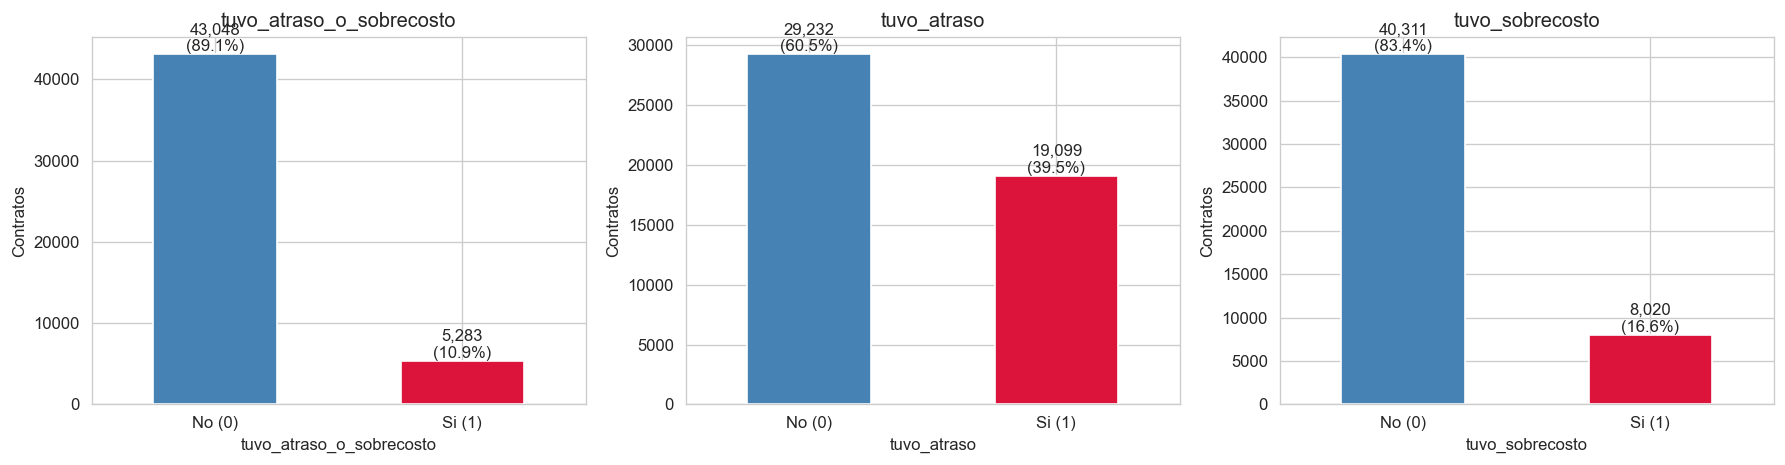
\includegraphics[width=0.95\textwidth]{01_balance_target.png}
\caption{Distribución de la variable objetivo \texttt{tuvo\_atraso}.}
\label{fig:balance_target}
\end{figure}

La distribución muestra un desbalance leve a moderado (60/40) que se considera
manejable para algoritmos de clasificación supervisada con técnicas estándar
de compensación, tales como \texttt{class\_weight = balanced} en modelos
lineales y de bosque, y \texttt{scale\_pos\_weight} en modelos de gradient
boosting.

\section{Comportamiento por modalidad de contratación}

La modalidad de contratación bajo la cual se adjudica un contrato muestra
diferencias sustantivas en las tasas observadas de atraso y sobrecosto, según
se observa en la Tabla \ref{tab:modalidad}.

\begin{table}[h!]
\centering
\caption{Tasas de atraso y sobrecosto por modalidad de contratación.}
\label{tab:modalidad}
\begin{tabular}{lccc}
\toprule
\textbf{Modalidad} & \textbf{Cantidad} & \textbf{Tasa atraso} & \textbf{Tasa sobrecosto} \\
\midrule
Selección Abreviada de Menor Cuantía & 12.932 & 55,7\,\% & 78,3\,\% \\
Contratación directa & 9.981 & 63,7\,\% & 93,4\,\% \\
Mínima cuantía & 9.747 & 76,2\,\% & 82,3\,\% \\
Licitación pública Obra Pública & 8.575 & 38,7\,\% & 75,1\,\% \\
Contratación régimen especial & 2.905 & 77,1\,\% & 91,8\,\% \\
\bottomrule
\end{tabular}
\end{table}

El hallazgo más relevante es que la Licitación Pública, modalidad percibida
como la más rigurosa y compleja administrativamente, es en realidad la que
presenta la \textbf{menor tasa de atraso} (38,7\,\%) de las cinco modalidades
principales. Por el contrario, las modalidades de menor cuantía (Mínima
Cuantía con 76,2\,\% y Contratación Directa con 63,7\,\%) son las que
presentan las tasas más altas de atraso.

Este resultado, aunque contraintuitivo en una primera lectura, es coherente
con la estructura del proceso contractual: la Licitación Pública involucra
mayores controles previos, mayores requisitos financieros sobre el proponente y
plazos de ejecución mejor planificados, lo que reduce la probabilidad de
imprevistos. Las modalidades de menor cuantía, en cambio, suelen aplicarse a
contratos de menor valor y de muy corta duración, donde un evento imprevisto
(retraso en el suministro, pérdidas climáticas) genera un atraso proporcional
mucho mayor.

\section{Comportamiento por nivel territorial y tipo de proponente}

La segregación por orden de la entidad contratante (nacional vs.\ territorial) y
por características del proponente arroja los resultados de la Tabla
\ref{tab:segmentos}.

\begin{table}[h!]
\centering
\caption{Tasas por segmento de entidad y de proponente.}
\label{tab:segmentos}
\begin{tabular}{lccc}
\toprule
\textbf{Segmento} & \textbf{n} & \textbf{Tasa atraso} & \textbf{Tasa sobrecosto} \\
\midrule
Orden Nacional & 15.667 & 55,9\,\% & 74,6\,\% \\
Orden Territorial & 32.016 & 62,6\,\% & 87,5\,\% \\
Proponente individual (no consorcio) & 37.702 & 65,0\,\% & 85,0\,\% \\
Consorcio o Unión Temporal & 10.629 & 44,6\,\% & 77,9\,\% \\
Pyme & 27.469 & 62,2\,\% & 80,8\,\% \\
No pyme & 20.862 & 58,2\,\% & 86,9\,\% \\
\bottomrule
\end{tabular}
\end{table}

Tres observaciones se desprenden de la tabla. Primero, los contratos
territoriales presentan mayor riesgo en ambas dimensiones que los nacionales,
patrón consistente con la heterogeneidad de capacidades técnicas entre
entidades departamentales y municipales. Segundo, los consorcios y uniones
temporales presentan tasas de atraso 20 puntos porcentuales por debajo de los
proponentes individuales (44,6\,\% vs.\ 65,0\,\%), sugiriendo que la
complementariedad de capacidades reduce el riesgo operativo. Tercero, la
distinción pyme/no pyme, aunque significativa, es de menor magnitud: las pymes
presentan apenas 4 puntos porcentuales más de atraso, pero menor sobrecosto,
lo cual sugiere que las pymes son más estrictas en el control financiero del
contrato aunque más vulnerables a desviaciones de plazo.

\section{Distribución geográfica}

La incidencia de modificaciones contractuales presenta una variación notable
entre departamentos. La Figura \ref{fig:tasa_depto} muestra la tasa de atraso
para los quince departamentos con mayor número de contratos de obra.

\begin{figure}[H]
\centering
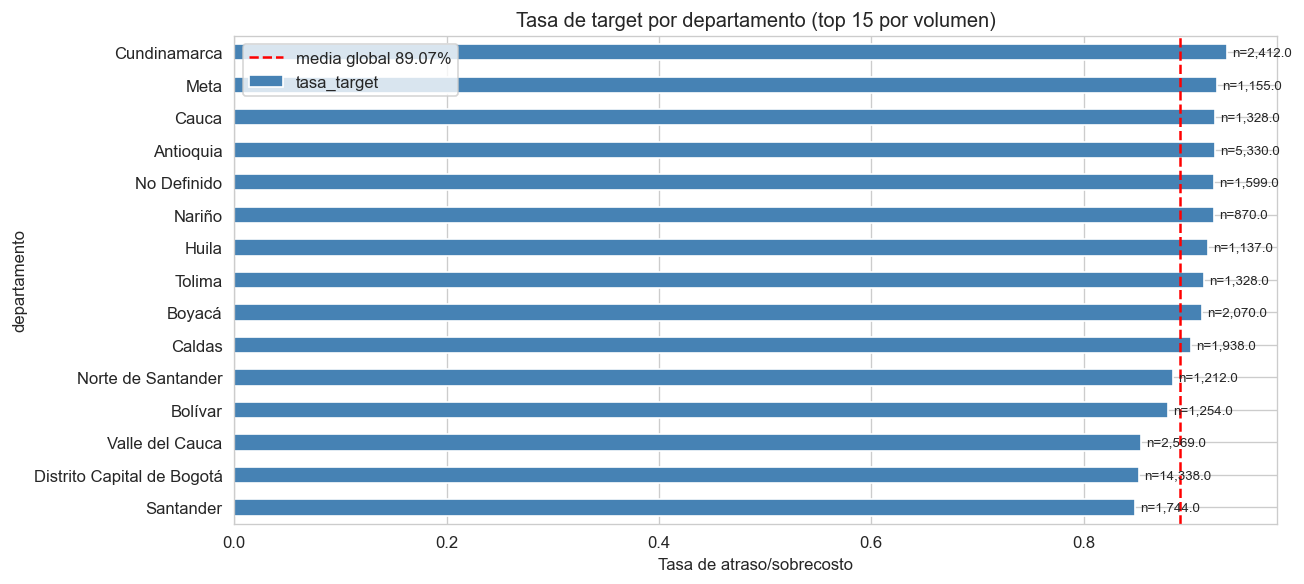
\includegraphics[width=0.95\textwidth]{02_tasa_por_depto.png}
\caption{Tasa de atraso por departamento (top 15 por volumen).}
\label{fig:tasa_depto}
\end{figure}

Antioquia presenta la tasa de atraso más alta entre los departamentos con
muestra significativa: 69,7\,\% sobre 5.330 contratos. Bogotá D.C.\ concentra
el mayor volumen de contratación (14.338 contratos) con una tasa de atraso
intermedia del 52,9\,\%. Valle del Cauca, Caldas y Cundinamarca presentan
tasas de atraso entre el 56\,\% y el 57\,\%, ligeramente por debajo del
promedio nacional. La categoría ``No Definido'' (1.599 contratos) presenta la
tasa más alta (76,2\,\%), confirmando que la ausencia de información
geográfica básica es, por sí misma, un indicador de problemas administrativos
en el contrato.

\section{Distribución por valor y duración planificada}

Un análisis cuartil del valor del contrato y de la duración planificada arroja
hallazgos significativos, presentados en las Tablas \ref{tab:cuartil_valor} y
\ref{tab:cuartil_duracion}.

\begin{table}[h!]
\centering
\caption{Tasas de atraso y sobrecosto por cuartil de valor del contrato.}
\label{tab:cuartil_valor}
\begin{tabular}{lccc}
\toprule
\textbf{Cuartil} & \textbf{Valor mediano} & \textbf{Tasa atraso} & \textbf{Tasa sobrecosto} \\
\midrule
Q1 (bajo) & \$27,7 M & 82,2\,\% & 91,6\,\% \\
Q2 & \$100 M & 68,5\,\% & 87,0\,\% \\
Q3 & \$401 M & 52,5\,\% & 80,5\,\% \\
Q4 (alto) & \$2.666 M & 38,6\,\% & 74,5\,\% \\
\bottomrule
\end{tabular}
\end{table}

\begin{table}[h!]
\centering
\caption{Tasas de atraso y sobrecosto por cuartil de duración planificada.}
\label{tab:cuartil_duracion}
\begin{tabular}{lccc}
\toprule
\textbf{Cuartil} & \textbf{Duración mediana} & \textbf{Tasa atraso} & \textbf{Tasa sobrecosto} \\
\midrule
Q1 (corta) & 29 días & 84,5\,\% & 88,8\,\% \\
Q2 & 80 días & 63,2\,\% & 82,9\,\% \\
Q3 & 168 días & 43,7\,\% & 77,6\,\% \\
Q4 (larga) & 401 días & 27,3\,\% & 74,7\,\% \\
\bottomrule
\end{tabular}
\end{table}

\begin{figure}[H]
\centering
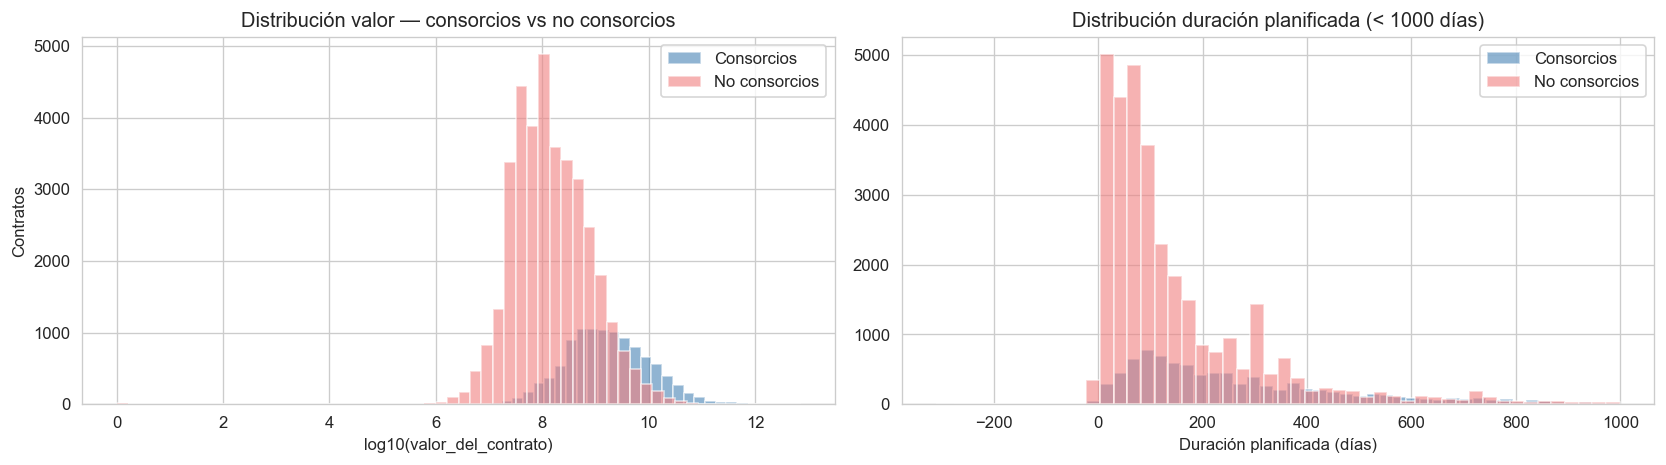
\includegraphics[width=0.95\textwidth]{15_valor_duracion.png}
\caption{Relación entre el valor y la duración del contrato con las tasas de modificación.}
\label{fig:valor_dur}
\end{figure}

Este resultado es uno de los más relevantes del estudio. La relación entre
valor o duración y riesgo es \textbf{inversa}: los contratos de menor valor y
menor duración son los que tienen mayor probabilidad de atraso. Tres
interpretaciones posibles, no excluyentes, justifican el hallazgo. Primero, el
sesgo de planificación: los contratos de gran valor y larga duración reciben
mayor planeación previa (estudios de pre-factibilidad, cronogramas detallados,
\emph{buffer} presupuestal), lo cual reduce el riesgo. Segundo, la definición
del evento: un atraso de pocos días en un contrato de 29 días es
proporcionalmente mucho mayor que el mismo atraso en uno de 400 días. Tercero,
la holgura de cronograma: los contratos largos suelen tener cronogramas con
holgura intrínseca que absorben pequeñas demoras sin necesidad de formalizar
una prórroga.

\section{Análisis de información mutua y permutación}

Para identificar las variables predictoras con mayor poder discriminativo
sobre los \emph{targets}, se calcularon dos métricas complementarias. La
Información Mutua mide la dependencia estadística entre cada variable y el
\emph{target}, sin asumir linealidad. La Importancia por Permutación mide
cuánto cae la métrica AUC del modelo cuando se permuta aleatoriamente una
variable, dejando todas las demás intactas.

La Figura \ref{fig:permutation} muestra la importancia por permutación para
las treinta variables más relevantes sobre el \emph{target}
\texttt{tuvo\_atraso}.

\begin{figure}[H]
\centering
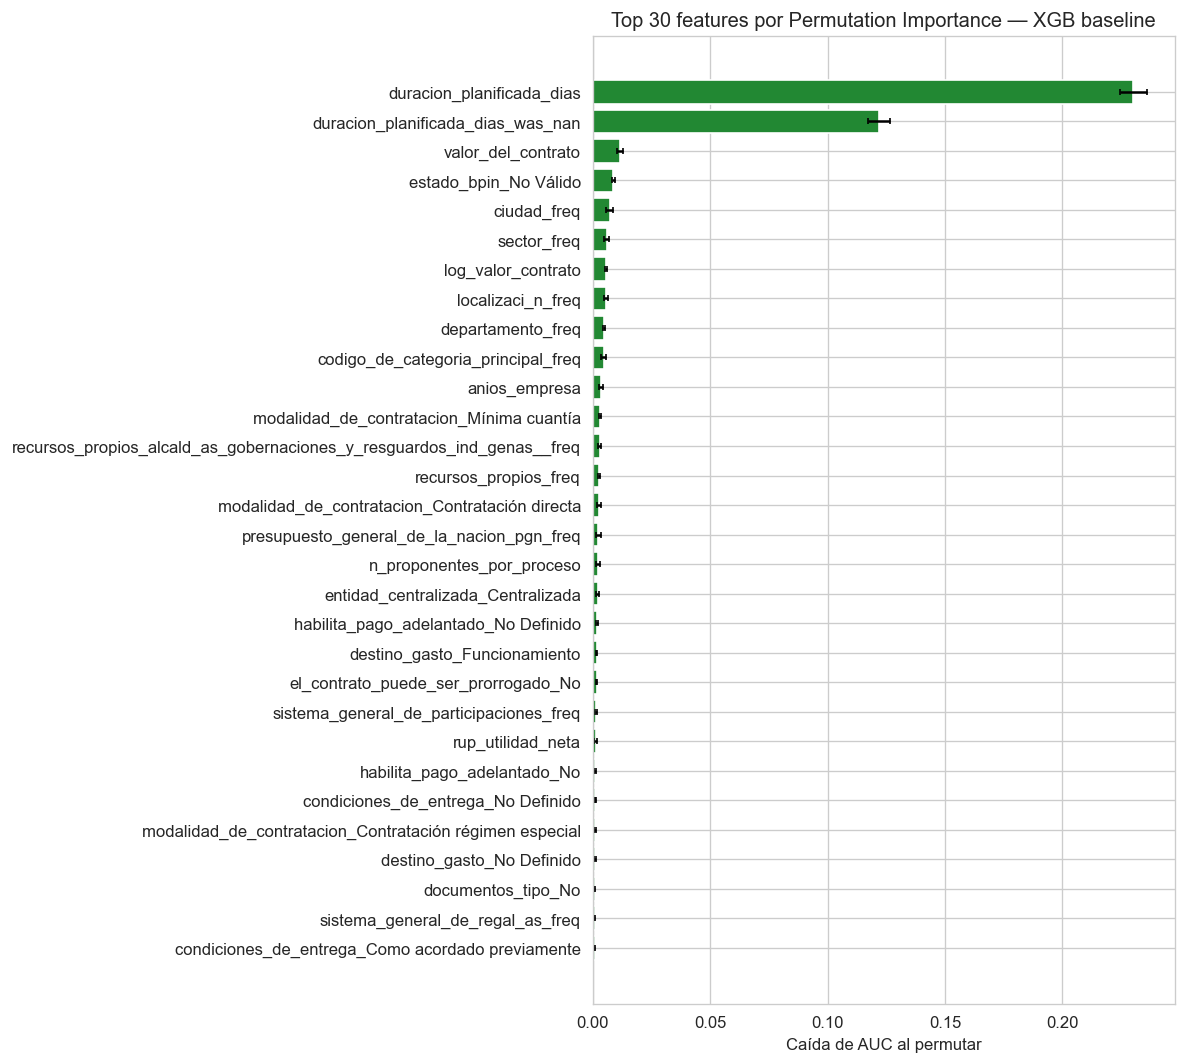
\includegraphics[width=0.95\textwidth]{22_permutation_top30.png}
\caption{Importancia por permutación de las 30 features con mayor impacto en el modelo.}
\label{fig:permutation}
\end{figure}

Los hallazgos centrales son los siguientes. La variable
\texttt{duracion\_planificada\_dias} domina ampliamente: su importancia por
permutación (0,230) es aproximadamente cinco veces mayor que la de la segunda
variable. El flag \texttt{duracion\_planificada\_dias\_was\_nan} aparece como
segundo predictor (0,122); es decir, el hecho de que un contrato no tenga
duración planificada registrada es, en sí mismo, una señal predictiva
importante. Las variables geográficas (\texttt{ciudad\_freq},
\texttt{localizaci\_n\_freq}, \texttt{departamento\_freq}) aparecen
consistentemente en el top 10, confirmando la relevancia de la dimensión
territorial. La variable \texttt{codigo\_de\_categoria\_principal\_freq}
(clasificación UNSPSC del objeto contractual) aporta señal predictiva sin
haber sido explotada en versiones iniciales del dataset.

\section{Hallazgos consolidados del análisis}

El análisis estadístico permite condensar las siguientes conclusiones
cuantitativas que orientan el modelado predictivo:

\begin{enumerate}
    \item La prevalencia de atraso en contratos de obra pública es de
    60,48\,\%. La de sobrecosto es de 83,41\,\%.
    \item El valor del contrato y la duración planificada son las variables
    predictoras más importantes. La relación es inversa: contratos pequeños y
    cortos tienen mayor probabilidad de atraso.
    \item La modalidad de contratación discrimina fuertemente. Licitación
    Pública es la menos riesgosa (38,7\,\% de atraso), Mínima Cuantía es la
    más riesgosa (76,2\,\%).
    \item Los consorcios presentan 20 puntos porcentuales menos de atraso que
    los proponentes individuales.
    \item La geografía tiene impacto significativo. Antioquia presenta la tasa
    más alta entre departamentos con muestra significativa (69,7\,\%); Caldas
    y Valle del Cauca presentan las más bajas entre los más grandes.
    \item Las variables estructurales del proveedor (RUP) aportan señal
    marginal. Su valor predictivo está limitado por la cobertura parcial y la
    redundancia con variables del contrato.
    \item Los indicadores del pliego no son predictivos como variables
    continuas, aunque el flag de ``pliego extraído / no extraído'' sí captura
    alguna señal residual relacionada con el tipo de proceso.
\end{enumerate}

% =====================================================================
% CAPÍTULO 3 — MODELO
% =====================================================================
\chapter{Elaboración del modelo predictivo}
\label{cap:modelo}

Este capítulo describe el proceso completo de construcción del modelo
predictivo, organizado conforme a las fases del marco CRISP-DM. El propósito
no es únicamente presentar los resultados finales, sino explicar la
justificación técnica de cada decisión tomada durante el proceso.

\section{Definición del problema de modelado}

El problema se formula como un problema de clasificación binaria supervisada
con dos variables objetivo simultáneas (\texttt{tuvo\_atraso} y
\texttt{tuvo\_sobrecosto}). La elección de clasificación binaria sobre
regresión se justifica porque la información de interés operativo para el
usuario final no es la magnitud del atraso o del sobrecosto, sino su
probabilidad de ocurrencia. Esta probabilidad permite priorizar contratos para
auditoría, asignar recursos de supervisión y comunicar el riesgo al empresario
en términos comprensibles.

\section{Identificación y exclusión de variables con fuga de información}

Antes de entrenar cualquier modelo fue necesario asegurar que ninguna de las
variables predictoras contuviera información que solo se conoce después de la
ejecución del contrato. Este fenómeno se conoce como \emph{data leakage} y, si
no se controla, produce modelos con métricas artificialmente altas que fallan
en producción. Se identificaron catorce variables prohibidas, organizadas en
cuatro categorías según se detalla en la Tabla \ref{tab:leakage}.

\begin{table}[h!]
\centering
\caption{Variables excluidas por riesgo de fuga de información temporal.}
\label{tab:leakage}
\small
\begin{tabular}{p{3.5cm}p{6cm}p{4.5cm}}
\toprule
\textbf{Categoría} & \textbf{Variables} & \textbf{Razón de exclusión} \\
\midrule
Targets directos & \texttt{tiempo}, \texttt{presupuesto}, \texttt{alcance} & Son los binarios fuente de los \emph{targets} \\
Conteos post-contractuales & \texttt{n\_modif\_general}, \texttt{n\_tipos\_distintos}, \texttt{n\_tipo\_no\_definido}, \texttt{n\_suspension} & Solo se conocen al cerrar la ejecución \\
Flags post-contractuales & \texttt{tiene\_cesion}, \texttt{tiene\_conclusion}, \texttt{tiene\_suspension} & Indican eventos durante la ejecución \\
Métricas temporales post & \texttt{dias\_adicionados}, \texttt{dias\_hasta\_primera\_adicion}, \texttt{ventana\_adiciones\_dias}, \texttt{ratio\_extension\_duracion} & Capturan información de la duración real \\
\bottomrule
\end{tabular}
\end{table}

\section{Preparación de los datos}

La preparación de datos sigue un pipeline lineal con cuatro pasos
secuenciales, cada uno con su propia justificación técnica: winsorización,
codificación de variables categóricas, imputación de valores ausentes y
división estratificada del dataset.

\subsection{Winsorización}

La winsorización consiste en reemplazar los valores por debajo del percentil 1
por el valor del percentil 1, y los valores por encima del percentil 99 por
el valor del percentil 99. Esta técnica neutraliza \emph{outliers} extremos
sin eliminar registros completos. Su uso se justifica por la presencia de
valores manifiestamente erróneos en los datos crudos (duraciones de millones
de días, valores de contrato del orden de $10^{13}$ pesos), atribuibles a
errores de carga en la plataforma SECOP.

\subsection{Codificación de variables categóricas}

Los algoritmos de \emph{Machine Learning} solo procesan entradas numéricas, lo
cual obliga a convertir las variables categóricas mediante alguna técnica de
codificación. La elección depende de la cardinalidad y la naturaleza de la
variable.

Se aplicó \textbf{One-Hot Encoding} para variables categóricas con
cardinalidad inferior a 20. La técnica crea una columna binaria por cada
categoría y es el estándar para categóricas nominales porque no impone un
orden artificial. Se aplicó \textbf{Frequency Encoding} para variables
categóricas con cardinalidad mayor o igual a 20. La técnica reemplaza cada
categoría por su frecuencia relativa en el dataset. Esta elección se justifica
para variables como \texttt{departamento} (32 valores), \texttt{ciudad} (más
de 1.000 valores) y \texttt{codigo\_de\_categoria\_principal} (1.506 valores
UNSPSC), donde el uso de One-Hot generaría una explosión dimensional que el
modelo no puede aprovechar.

Se descartaron dos alternativas evaluadas. El \emph{Label Encoding} se
descartó porque inyecta un orden artificial entre categorías que el modelo
lineal interpreta incorrectamente como una relación numérica. El \emph{Target
Encoding} se descartó por riesgo de fuga de información si no se calcula con
validación cruzada interna, aunque se mantiene como opción para iteraciones
futuras.

\subsection{Imputación con preservación del patrón de ausencia}

El dataset presenta valores ausentes en variables provenientes del RUP
(cobertura 49\,\%) y los indicadores de pliego (cobertura 8--37\,\%). Se
evaluaron cuatro estrategias mediante un experimento controlado, cuyos
resultados se resumen en la Tabla \ref{tab:imputacion}.

\begin{table}[h!]
\centering
\caption{Comparativa de estrategias de imputación según AUC sobre prueba.}
\label{tab:imputacion}
\begin{tabular}{lcc}
\toprule
\textbf{Estrategia} & \textbf{AUC test} & \textbf{Tiempo} \\
\midrule
\textbf{Mediana + flag \texttt{\_was\_nan}} & \textbf{0,8542} & 0,02 s \\
K-Nearest Neighbors (k=5) & 0,8093 & 6,09 s \\
MICE con Bayesian Ridge & 0,8066 & 44,32 s \\
MICE con Random Forest & 0,8015 & 33,65 s \\
\bottomrule
\end{tabular}
\end{table}

Contra la intuición de que los métodos sofisticados deberían producir mejores
resultados, la estrategia más simple (mediana acompañada de un indicador
binario que señala si el valor era originalmente \texttt{NaN}) obtuvo el mejor
AUC por un margen de 0,045 puntos. El motivo es que el patrón de ausencia es
informativo en sí mismo: que un contrato no tenga indicador financiero de
pliego extraído está correlacionado con su modalidad y tipo de entidad
contratante. Los métodos sofisticados, al ``tapar el hueco'' con un valor
plausible, eliminan esa señal residual de ausencia.

\subsection{División train/test estratificada}

Se aplicó una división 80/20 estratificada sobre la variable
\texttt{tuvo\_atraso}, con semilla aleatoria fija
(\texttt{random\_state = 42}). La estratificación garantiza que la
proporción de la clase positiva (60,48\,\%) se preserve exactamente en ambos
subconjuntos, según se observa en la Figura \ref{fig:balance_split}.

\begin{figure}[H]
\centering
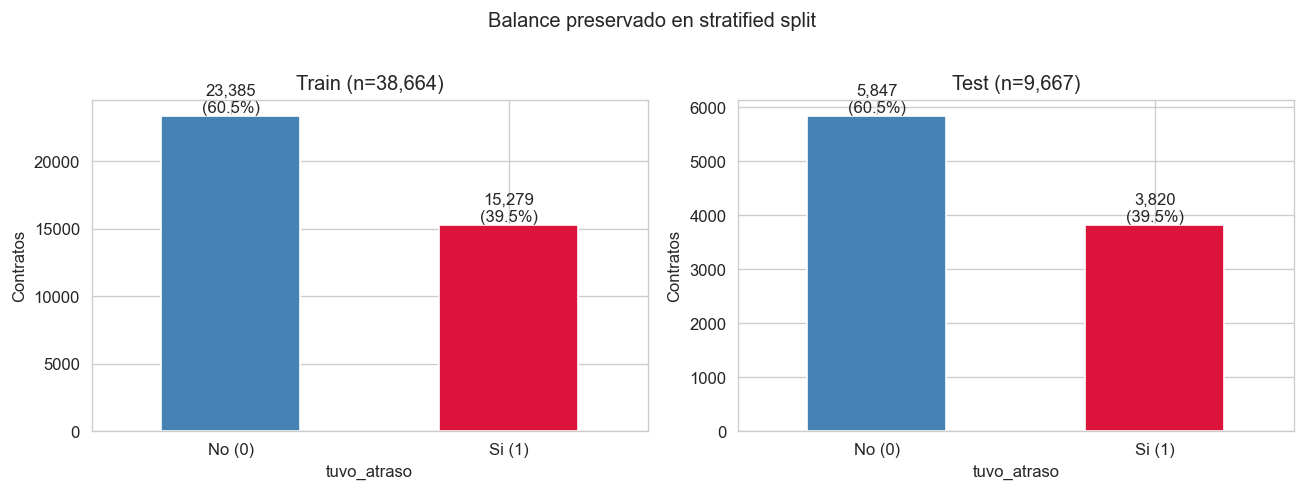
\includegraphics[width=0.95\textwidth]{04_balance_split.png}
\caption{Preservación del balance de la variable objetivo tras la división estratificada.}
\label{fig:balance_split}
\end{figure}

El conjunto de prueba se mantiene intocado durante toda la fase de
entrenamiento, selección de variables y calibración de hiperparámetros. Solo
se utiliza para la evaluación final del modelo ganador.

\section{Selección automatizada de variables}

El conjunto de entrada al modelado, tras el \emph{encoding}, alcanzó 152
variables predictoras. Para identificar las variables verdaderamente
relevantes, se aplicó una cascada de cuatro métodos complementarios: umbral
de varianza, filtro por correlación, importancia por permutación y
eliminación recursiva con validación cruzada (RFECV). La intersección de las
variables sobrevivientes a los métodos 3 y 4 constituyó el conjunto final de
30 variables seleccionadas.

\begin{figure}[H]
\centering
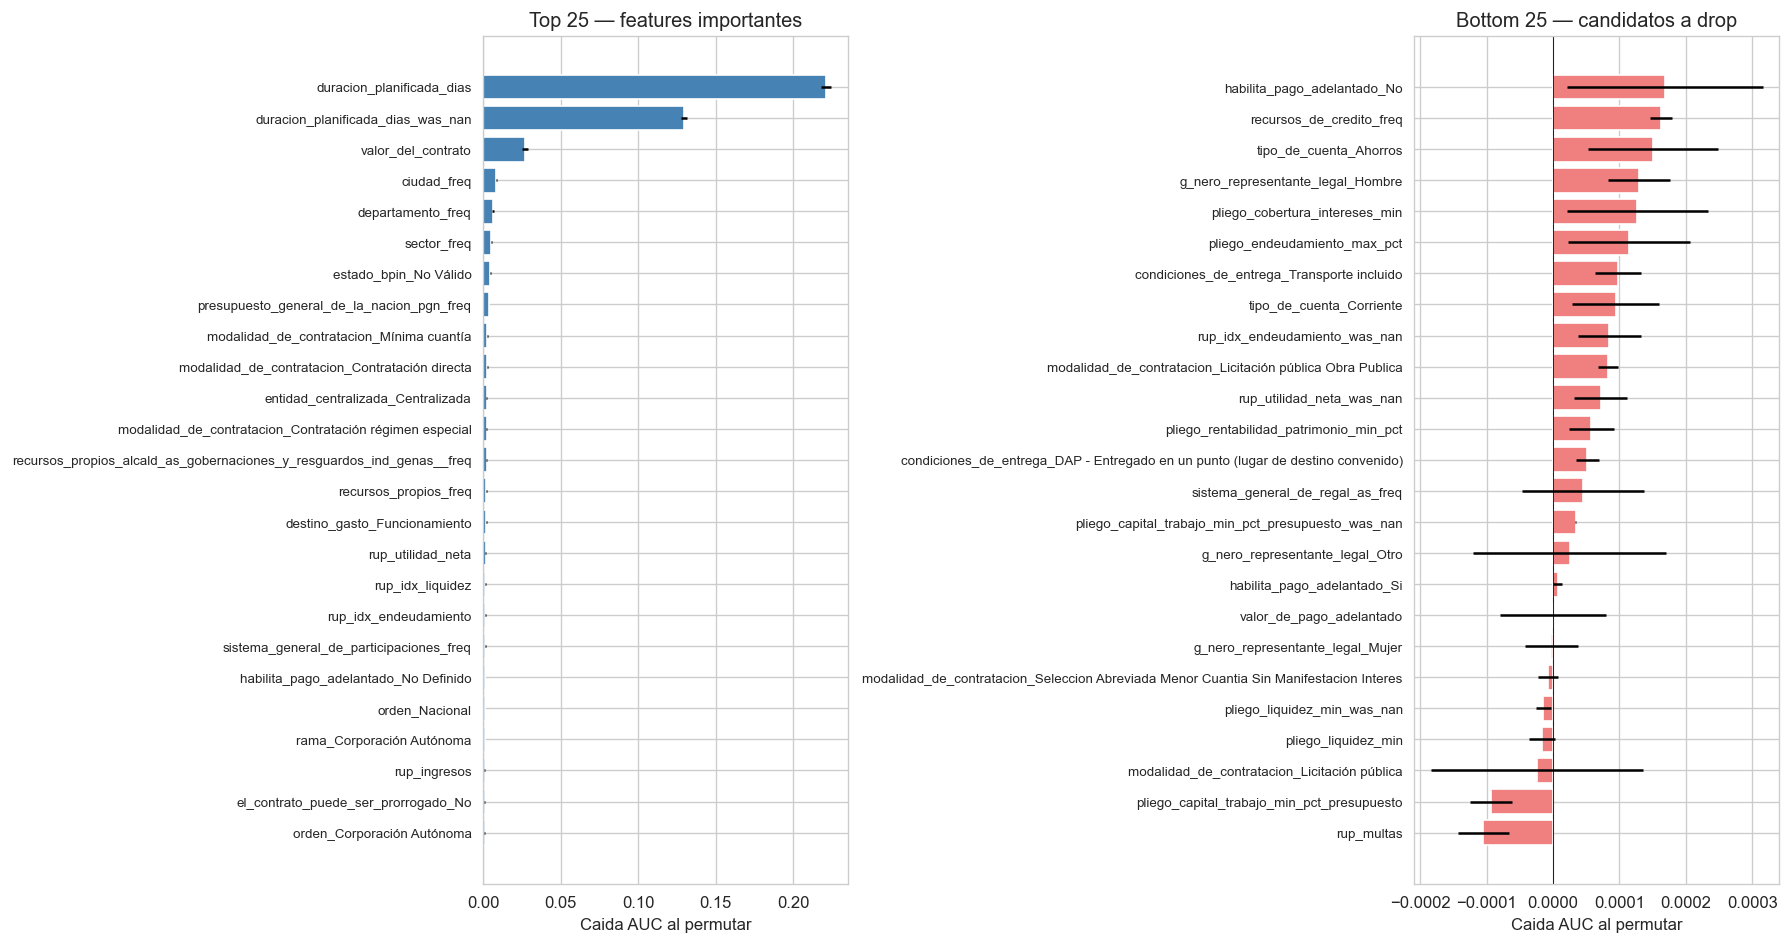
\includegraphics[width=0.95\textwidth]{09_permutation_importance.png}
\caption{Importancia por permutación de las features seleccionadas.}
\label{fig:perm_select}
\end{figure}

\begin{figure}[H]
\centering
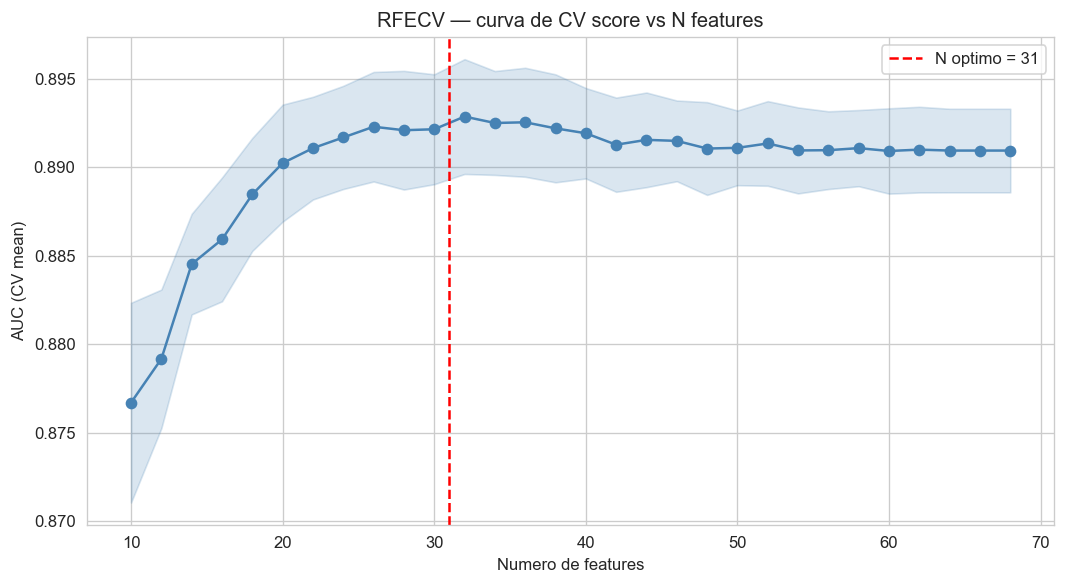
\includegraphics[width=0.95\textwidth]{10_rfecv_curve.png}
\caption{Curva de RFECV mostrando estabilización del desempeño con 30 variables.}
\label{fig:rfecv}
\end{figure}

El resultado de aplicar la selección de variables fue una mejora marginal
pero consistente del desempeño respecto al modelo con todas las variables,
según se ilustra en la Figura \ref{fig:reduccion}.

\begin{figure}[H]
\centering
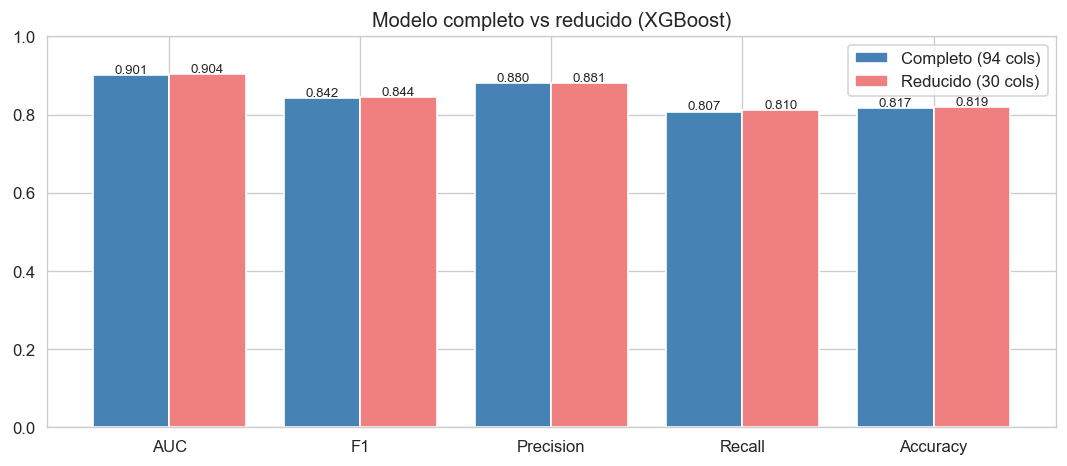
\includegraphics[width=0.95\textwidth]{11_comparativa_reduccion.png}
\caption{Comparativa de desempeño con y sin selección automatizada de variables.}
\label{fig:reduccion}
\end{figure}

\section{El zoológico de algoritmos}

Siguiendo la recomendación metodológica del codirector de cubrir el espectro
de familias de algoritmos para tener evidencia empírica robusta, se
entrenaron ocho modelos supervisados representativos de las principales
familias de clasificación, según se resume en la Tabla \ref{tab:zoologico}.

\begin{table}[h!]
\centering
\caption{Algoritmos evaluados en el zoológico de modelos.}
\label{tab:zoologico}
\begin{tabular}{lll}
\toprule
\textbf{Familia} & \textbf{Algoritmo} & \textbf{Escalado requerido} \\
\midrule
Lineal & Logistic Regression (LR) & Sí \\
Distancia & K-Nearest Neighbors (KNN) & Sí \\
Margen & Support Vector Machine (SVM lineal) & Sí \\
Bagging & Random Forest (RF) & No \\
Boosting & XGBoost & No \\
Boosting & LightGBM & No \\
Probabilístico & Gaussian Naive Bayes (NB) & Sí \\
Red neuronal & Multi-Layer Perceptron (MLP) & Sí \\
\bottomrule
\end{tabular}
\end{table}

Para cada algoritmo se ejecutó \texttt{RandomizedSearchCV} con entre 12 y 50
iteraciones por modelo, validación cruzada estratificada de 5 particiones y
optimización del Área Bajo la Curva ROC. La elección de
\texttt{RandomizedSearchCV} sobre \texttt{GridSearchCV} responde a un criterio
de eficiencia computacional, dado que el espacio de búsqueda incluye
variables continuas (tasa de aprendizaje, fracción de submuestreo) donde una
búsqueda exhaustiva sería prohibitiva.

Los algoritmos que requieren features en escala homogénea (LR, KNN, SVM, NB,
MLP) recibieron los datos previamente escalados con \texttt{StandardScaler}.
Los algoritmos basados en árboles (RF, XGBoost, LightGBM) operan directamente
sobre las features sin escalar, dado que sus \emph{splits} son comparaciones
binarias insensibles a la escala.

\subsection{Resultados sobre tuvo\_atraso}

Los ocho modelos del zoológico fueron evaluados sobre el conjunto de prueba
(9.667 contratos no vistos durante el entrenamiento). Los resultados se
presentan en la Tabla \ref{tab:resultados_zoo}, ordenados por AUC test
descendente.

\begin{table}[h!]
\centering
\caption{Resultados del zoológico de algoritmos sobre el conjunto de prueba.}
\label{tab:resultados_zoo}
\small
\begin{tabular}{lcccccc}
\toprule
\textbf{Modelo} & \textbf{AUC} & \textbf{F1} & \textbf{Precisión} & \textbf{Recall} & \textbf{Exactitud} & \textbf{Tiempo} \\
\midrule
\textbf{LightGBM} & \textbf{0,9091} & 0,8503 & 0,8672 & 0,8341 & 0,8268 & 380 s \\
XGBoost & 0,9069 & 0,8500 & 0,8765 & 0,8250 & 0,8238 & 186 s \\
Random Forest & 0,8996 & 0,8489 & 0,8262 & 0,8729 & 0,8120 & 368 s \\
MLP & 0,8630 & 0,8263 & 0,8147 & 0,8382 & 0,7868 & 86 s \\
Logistic Regression & 0,8402 & 0,7982 & 0,8243 & 0,7737 & 0,7634 & 93 s \\
SVM lineal & 0,8381 & 0,8144 & 0,7705 & 0,8635 & 0,7619 & 223 s \\
KNN & 0,8333 & 0,8077 & 0,7565 & 0,8663 & 0,7505 & 176 s \\
Naive Bayes & 0,7519 & 0,3482 & 0,9952 & 0,2110 & 0,5222 & 8 s \\
\bottomrule
\end{tabular}
\end{table}

\begin{figure}[H]
\centering
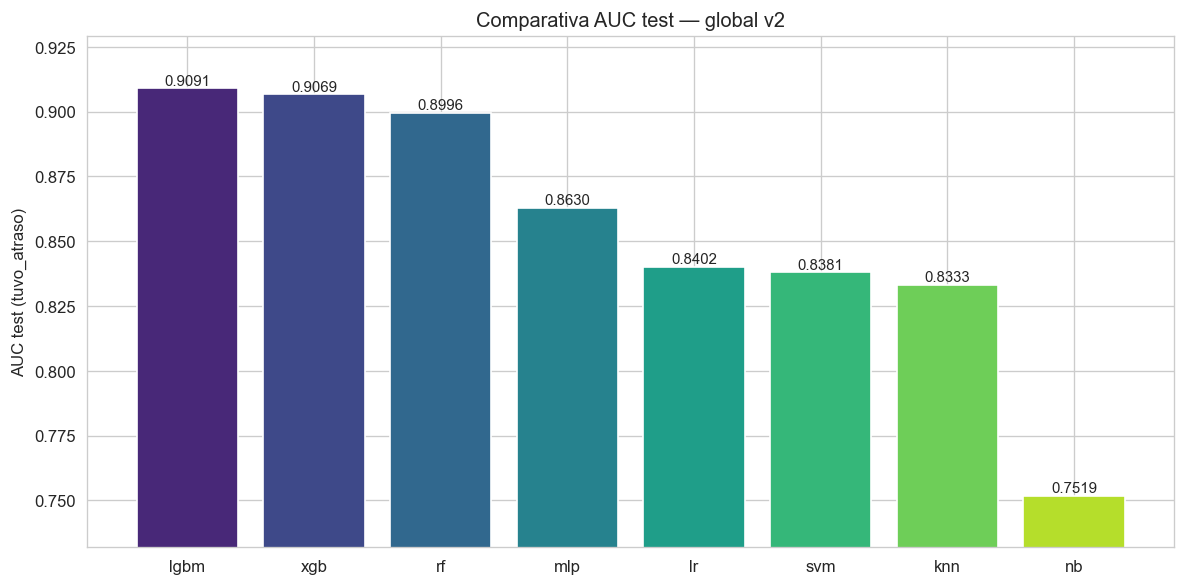
\includegraphics[width=0.95\textwidth]{23_comparativa_auc.png}
\caption{Comparativa del Área Bajo la Curva ROC entre los ocho algoritmos.}
\label{fig:auc_zoo}
\end{figure}

\begin{figure}[H]
\centering
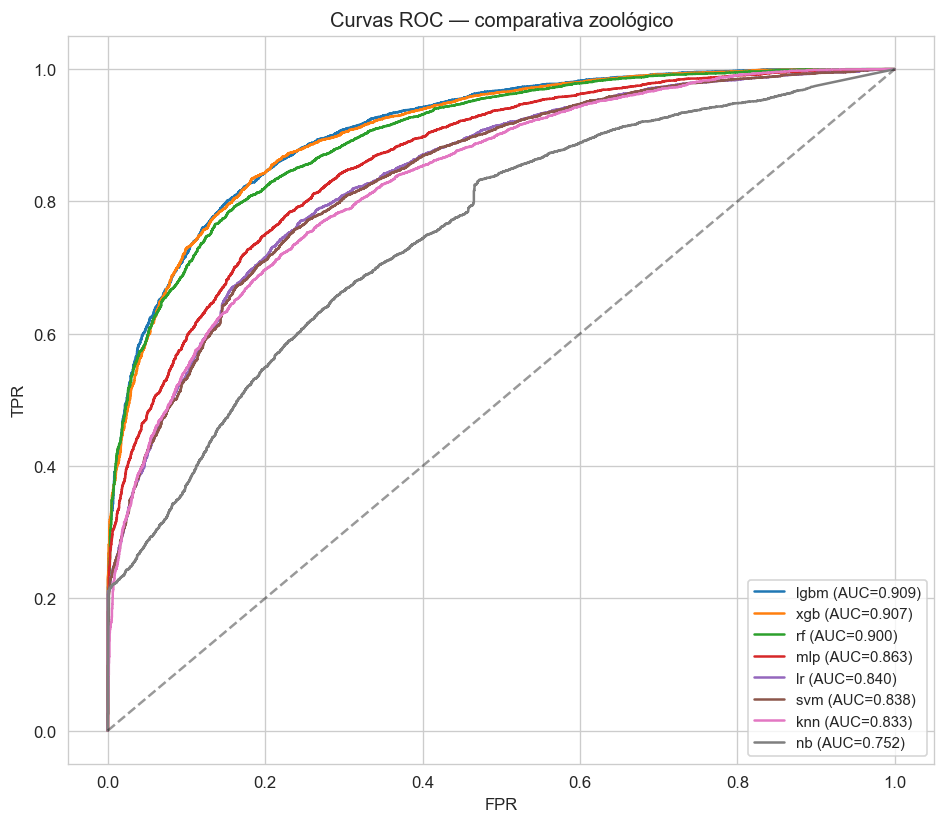
\includegraphics[width=0.95\textwidth]{24_curvas_roc.png}
\caption{Curvas ROC comparativas de los ocho algoritmos sobre el conjunto de prueba.}
\label{fig:roc_zoo}
\end{figure}

\begin{figure}[H]
\centering
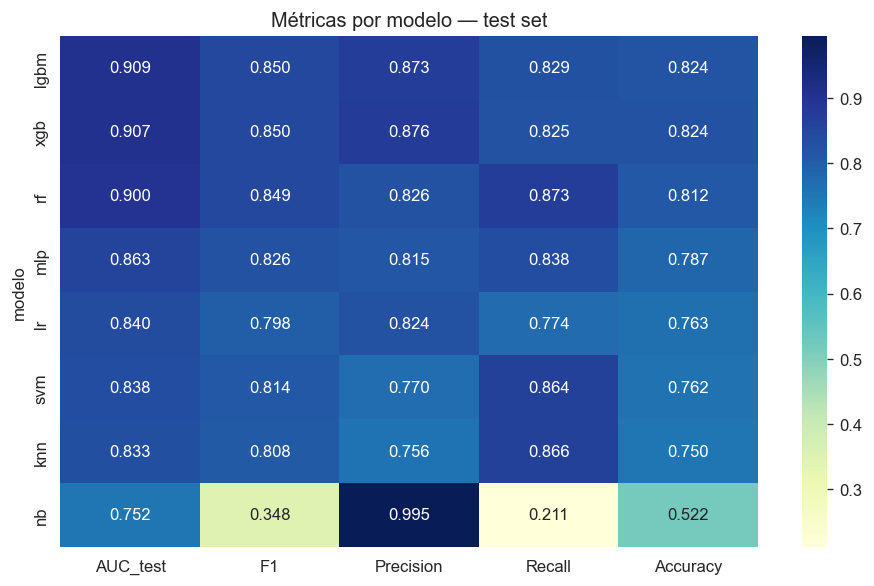
\includegraphics[width=0.95\textwidth]{25_heatmap_metricas.png}
\caption{Mapa de calor de métricas por modelo sobre el conjunto de prueba.}
\label{fig:heatmap_metricas}
\end{figure}

\subsection{Interpretación de los resultados}

Los resultados confirman patrones documentados en la literatura sobre datos
tabulares. Los modelos de \emph{boosting} (LightGBM y XGBoost) dominan
ampliamente, con AUC en torno a 0,91 y diferencia entre sí de apenas 0,0022.
Random Forest queda en tercer lugar (AUC 0,8996), apenas un punto porcentual
por debajo del \emph{boosting}. Las redes neuronales (MLP) quedan en cuarto
lugar (AUC 0,8630), resultado consistente con la literatura sobre datos
tabulares de tamaño moderado. Los modelos lineales (LR, SVM lineal) rondan
AUC 0,84, lo cual confirma que el problema tiene relaciones no lineales que
un modelo lineal no captura. \emph{Naive Bayes} presenta el peor desempeño
con un patrón patológico: precisión casi perfecta (99,5\,\%) pero
\emph{recall} extremadamente bajo (21,1\,\%), debido a la violación de la
asunción de independencia condicional entre features.

\subsection{Matriz de confusión del modelo ganador}

La matriz de confusión del LightGBM ganador sobre el conjunto de prueba, con
umbral de decisión 0,50, se presenta en la Figura \ref{fig:cm_lgbm}.

\begin{figure}[H]
\centering
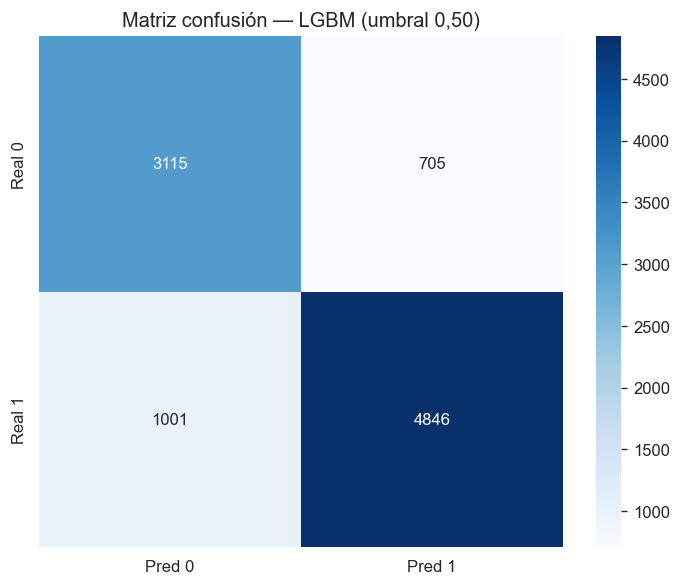
\includegraphics[width=0.85\textwidth]{26_matriz_confusion_lgbm.png}
\caption{Matriz de confusión del modelo LightGBM sobre el conjunto de prueba.}
\label{fig:cm_lgbm}
\end{figure}

El balance entre falsos positivos y falsos negativos es razonable. El modelo
prioriza ligeramente la captura de positivos reales (\emph{recall} 83,4\,\%)
sobre la precisión (86,7\,\%), lo cual es deseable en un sistema de alerta
temprana.

\section{Experimentación con cuatro estrategias de tuning}

Para profundizar la calibración del modelo se ejecutó un experimento
adicional comparando cuatro estrategias de búsqueda de hiperparámetros sobre
XGBoost, según se presenta en la Tabla \ref{tab:tuning}.

\begin{table}[h!]
\centering
\caption{Comparativa de cuatro estrategias de tuning de hiperparámetros.}
\label{tab:tuning}
\begin{tabular}{lccc}
\toprule
\textbf{Estrategia} & \textbf{CV AUC} & \textbf{Desv. estándar} & \textbf{Tiempo} \\
\midrule
\textbf{Grid Search reducido} & 0,9101 & \textbf{0,0026} & 435 s \\
Bayesian Optimization (Optuna TPE) & 0,9103 & 0,0026 & 329 s \\
Random Search & 0,9089 & 0,0027 & 88 s \\
Halving Random Search & 0,8293 & 0,0234 & 10 s \\
\bottomrule
\end{tabular}
\end{table}

Grid Search y Bayesian Optimization empatan virtualmente en CV AUC, pero el
Grid manual presenta menor desviación estándar entre particiones, lo cual
indica mayor estabilidad. Halving Random Search fracasó en este problema:
descartó tempranamente configuraciones que requerían más datos para mostrar
su verdadero valor, confirmando una limitación conocida del método.

\section{Arquitectura multi-target}

Dado que el segundo objetivo específico del proyecto exige predecir tanto
atrasos como sobrecostos, se evaluaron dos arquitecturas alternativas: dos
modelos separados o un modelo multi-target en un único pipeline. Los
resultados se ilustran en la Figura \ref{fig:multi_single}.

\begin{figure}[H]
\centering
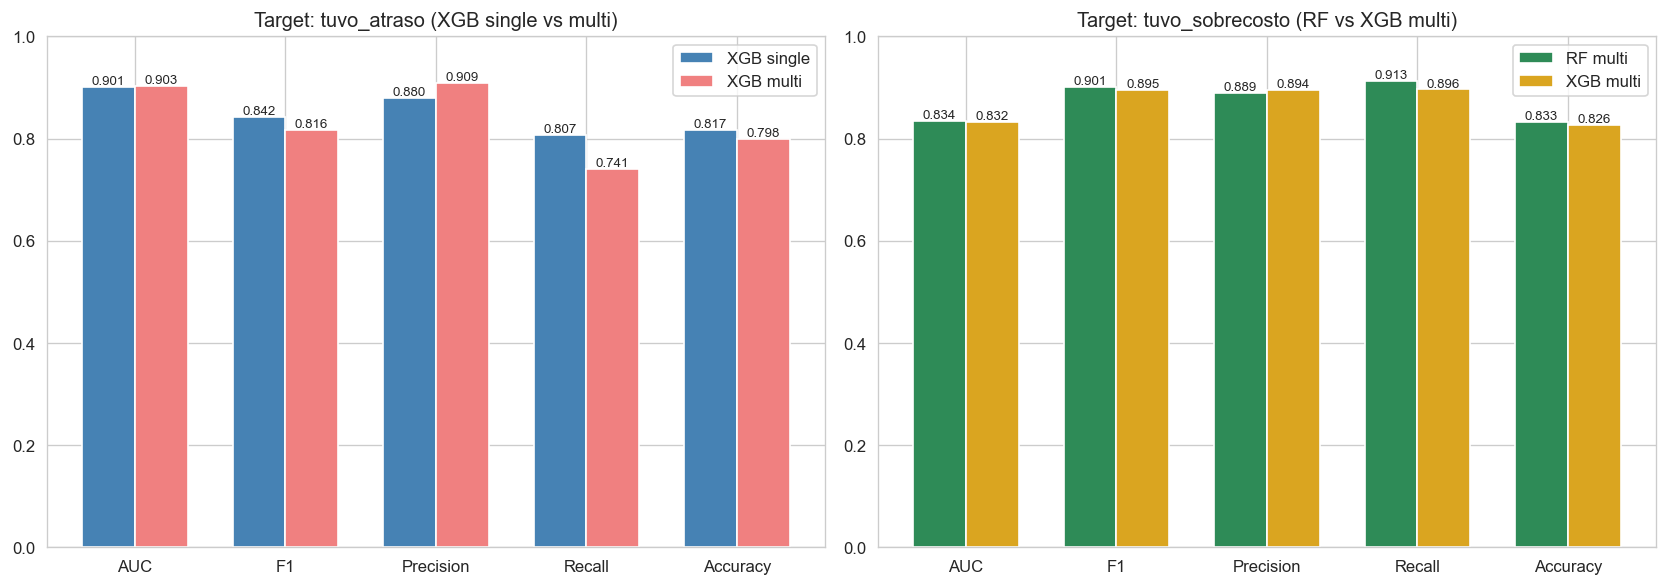
\includegraphics[width=0.95\textwidth]{12_multi_vs_single.png}
\caption{Comparativa de desempeño entre arquitectura single-target y multi-target.}
\label{fig:multi_single}
\end{figure}

El resultado es que la arquitectura multi-target no degrada el desempeño y,
en el caso del Random Forest, lo mejora marginalmente. La arquitectura
multi-target tiene ventajas operativas adicionales: simplifica el pipeline de
inferencia, reduce el costo de mantenimiento y garantiza que las predicciones
de ambos targets se realicen con el mismo vector de variables de entrada.

\begin{figure}[H]
\centering
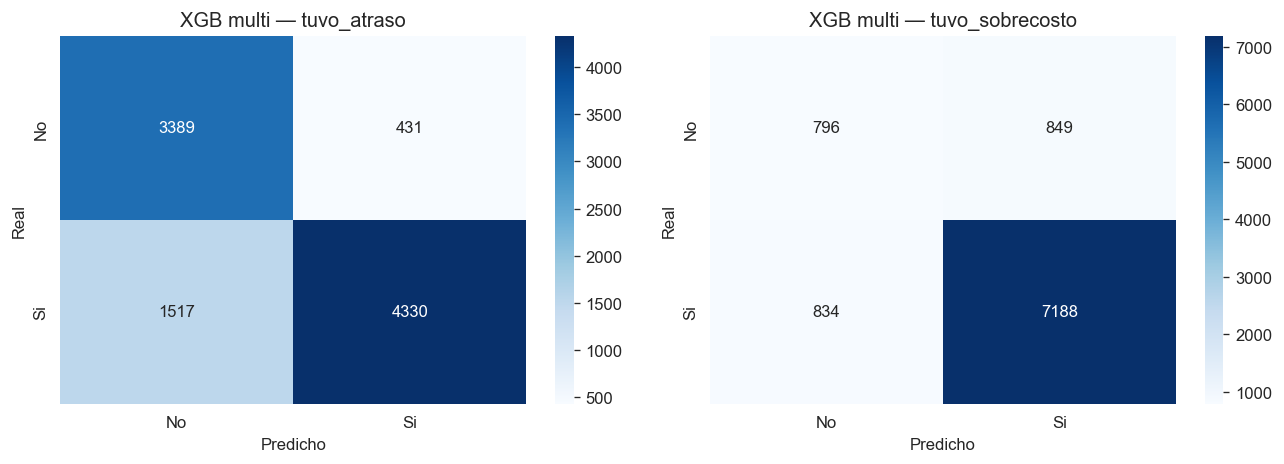
\includegraphics[width=0.95\textwidth]{13_cm_multi.png}
\caption{Matrices de confusión del modelo multi-target sobre los dos targets.}
\label{fig:cm_multi}
\end{figure}

\section{Validación y comparativa entre versiones}

Para garantizar la no-trivialidad de los resultados, se aplicaron tres
verificaciones independientes. La comparación contra clasificador trivial
muestra que un modelo que siempre predice la clase mayoritaria obtendría
exactitud del 60,5\,\% sobre \texttt{tuvo\_atraso}, mientras que el modelo
ganador alcanza exactitud del 82,7\,\%. La consistencia entre algoritmos
independientes (RF, XGBoost y LightGBM convergen a AUC en torno a 0,90)
sugiere que la señal capturada es real. La verificación empírica de
no-leakage confirma que ninguna de las catorce variables identificadas como
\emph{leakage} aparece entre las 30 variables más importantes seleccionadas.

El proyecto desarrolló dos versiones del modelo predictivo, cuya comparativa
se presenta en la Tabla \ref{tab:v1_v2}.

\begin{table}[h!]
\centering
\caption{Comparativa entre las dos versiones del modelo predictivo.}
\label{tab:v1_v2}
\begin{tabular}{llcc}
\toprule
\textbf{Versión} & \textbf{Target} & \textbf{AUC} & \textbf{F1} \\
\midrule
v1 XGBoost tuneado & \texttt{tuvo\_atraso} & 0,9088 & 0,8522 \\
\textbf{v2 LightGBM} & \texttt{tuvo\_atraso} & \textbf{0,9091} & 0,8503 \\
v1 XGBoost tuneado & \texttt{tuvo\_sobrecosto} & 0,8358 & 0,8508 \\
\textbf{v2 LightGBM} & \texttt{tuvo\_sobrecosto} & 0,8338 & \textbf{0,8731} \\
\bottomrule
\end{tabular}
\end{table}

La mejora en AUC de atraso es marginal (+0,0003); el F1 de sobrecosto mejora
en 0,022 puntos. La conclusión empírica es que las variables estructurales
del proveedor aportan información predictiva muy limitada. A pesar de la
mejora marginal, se selecciona \textbf{LightGBM v2} como modelo final del
proyecto por tres razones: mayor completitud metodológica, F1 superior en
sobrecosto y fundamento para iteraciones futuras.

\section{Síntesis del capítulo}

El proceso de construcción del modelo predictivo se desarrolló de manera
iterativa según los principios de CRISP-DM, con justificación técnica
explícita en cada decisión. Los resultados finales son: modelo seleccionado
LightGBM con calibración fina, AUC sobre prueba de 0,9091 para atraso y
0,8338 para sobrecosto, F1 de 0,8503 y 0,8731 respectivamente, 30 variables
predictoras seleccionadas mediante cascada de cuatro métodos.

% =====================================================================
% CAPÍTULO 4 — CHATBOT
% =====================================================================
\chapter{Prototipo de chatbot conversacional}
\label{cap:chatbot}

Este capítulo documenta el desarrollo del prototipo de interfaz de consulta
inteligente que da cumplimiento al cuarto objetivo específico del proyecto.
El prototipo se denomina Consultor de Riesgo Contractual y permite a un
empresario evaluar, mediante una conversación en lenguaje natural, el riesgo
histórico asociado a un contrato de obra pública que esté considerando
ejecutar.

\section{Caso de uso objetivo}

El usuario final del prototipo es un empresario o representante legal de una
empresa colombiana que está evaluando si participar en una licitación de obra
pública. Su pregunta natural es del tipo: ``Soy una microempresa de
construcción en Medellín, con 8 años de antigüedad y 25 empleados. Quiero
participar en una licitación pública de obra para construir un colegio, valor
4.500 millones COP, plazo de 18 meses, iría como consorcio con otra empresa.
¿Qué probabilidad tengo de cumplir el contrato sin atrasos?''.

El prototipo debe recibir esa descripción en texto libre, extraer las
variables del contrato y del perfil de la empresa, generar una predicción de
probabilidad de atraso y sobrecosto, identificar los factores principales que
influyen en la predicción, y comunicar el resultado en términos comprensibles
con recomendaciones contextuales y advirtiendo sobre las limitaciones del
modelo.

\section{Decisión arquitectónica: function calling}

El cuarto objetivo específico originalmente planteaba la implementación de un
sistema basado en agentes RAG (\emph{Retrieval Augmented Generation}) y
Grandes Modelos de Lenguaje. Tras analizar el caso de uso, se identificó que
una arquitectura RAG completa resultaba innecesaria para este prototipo. El
sistema no requiere consultar una base de conocimiento externa para generar
la respuesta: el conocimiento predictivo está enteramente en el modelo de
\emph{Machine Learning} entrenado.

Por este motivo, se adoptó una arquitectura más simple y apropiada:
\emph{function calling}. En este patrón, el modelo de lenguaje recibe la
declaración formal de una función disponible (\texttt{predecir\_riesgo}) y
decide, con base en el contexto de la conversación, cuándo y con qué
argumentos invocarla. La función se ejecuta del lado del backend (Python) y
devuelve el resultado al modelo de lenguaje, que lo humaniza para el usuario
final. Esta decisión no excluye la implementación posterior de una
arquitectura RAG completa.

\section{Arquitectura del prototipo}

El sistema completo se organiza en cuatro componentes principales:

\begin{enumerate}
    \item \textbf{Usuario}: ingresa una descripción en lenguaje natural sobre
    el contrato y su perfil.
    \item \textbf{Gemini 2.5 Flash}: extrae las variables del texto, decide
    invocar la función predictiva y humaniza el resultado.
    \item \textbf{Predictor (Python)}: normaliza el diccionario de entrada,
    aplica el pipeline completo de preprocesamiento, invoca el modelo
    LightGBM y calcula explicabilidad local con SHAP.
    \item \textbf{Modelo LightGBM}: ejecuta la predicción y devuelve las
    probabilidades de atraso y sobrecosto.
\end{enumerate}

\section{Componentes implementados}

El código del prototipo se organiza en cinco archivos principales, ubicados
en \texttt{modelo\_predictivo\_global/chatbot/}. El archivo
\texttt{predictor.py} encapsula la lógica de inferencia, cargando al iniciar
el modelo serializado y los artefactos de preprocesamiento. El archivo
\texttt{prompts.py} define el \emph{prompt} de sistema que indica al modelo
de lenguaje cómo debe comportarse. El archivo \texttt{gemini\_client.py}
implementa el cliente del modelo de lenguaje y el bucle de \emph{function
calling}. El archivo \texttt{app.py} implementa una interfaz web mediante
Streamlit. Finalmente, los archivos \texttt{README.md} y
\texttt{requirements.txt} documentan el uso del prototipo y las dependencias
necesarias.

\section{Modelo de lenguaje utilizado}

Se utilizó Gemini 2.5 Flash de Google, accedido mediante la API gratuita de
AI Studio. Las razones de esta elección son la disponibilidad con cuota
gratuita suficiente para un prototipo académico, el soporte de
\emph{function calling}, la coherencia con el resto del proyecto (el modelo
\texttt{gemini-2.5-flash-lite} ya se había integrado en el pipeline de
extracción de indicadores de pliego) y la velocidad y costo competitivos.

\section{Explicabilidad mediante SHAP}

Las predicciones se acompañan de los tres factores principales que más
empujaron la probabilidad hacia la clase positiva o negativa. Esto se calcula
mediante valores SHAP (\emph{SHapley Additive exPlanations}), una técnica
derivada de la teoría de juegos cooperativa que asigna a cada \emph{feature}
una contribución numérica a la predicción específica de un caso. La
implementación utiliza \texttt{shap.TreeExplainer}, optimizado para modelos
basados en árboles.

\section{Ejemplo de interacción}

A continuación se presenta un ejemplo real de conversación con el prototipo:

\begin{quote}
\textbf{Usuario}: Hola. Soy una microempresa de construcción en Bogotá. Quiero
participar en una licitación pública de obra para una vía urbana por 2 mil
millones COP con duración de 12 meses. Soy pyme y no me asocio con otros.
¿Qué riesgo tengo?

\textbf{Bot}: Análisis del contrato propuesto. Probabilidad de atraso en
plazo: 12,18\,\%. Probabilidad de adición presupuestal: 50,90\,\%. Factores
principales identificados: la duración planificada de 360 días reduce la
probabilidad de atraso porque está por encima del promedio de contratos
similares. La frecuencia de contratos en Bogotá aumenta ligeramente la
probabilidad de sobrecosto. Recomendaciones: dada la alta probabilidad de
sobrecosto, planifique el presupuesto con detalle e incluya contingencias
financieras. Aunque la probabilidad de atraso es baja, mantenga un plan de
trabajo robusto. Limitaciones: el modelo no predice si su empresa será
adjudicada ni evalúa la capacidad técnica específica.
\end{quote}

\section{Limitaciones del prototipo}

El prototipo es funcional y demuestra la viabilidad del concepto, pero
presenta limitaciones que se documentan explícitamente. Las probabilidades no
están calibradas formalmente (Platt scaling o regresión isotónica). Las
categorías no vistas durante el entrenamiento se tratan como categoría
desconocida (frecuencia 0), lo cual puede generar predicciones poco
confiables para territorios poco frecuentes. Las conversaciones no se
persisten entre sesiones. El modelo no predice si la empresa será
adjudicada, sino el comportamiento histórico de contratos similares.
Finalmente, las únicas variables del perfil del proponente son
\texttt{es\_pyme} y \texttt{es\_grupo}; el modelo no conoce la experiencia
previa de la empresa ni la composición de su equipo técnico.

\section{Síntesis del capítulo}

El prototipo de \emph{chatbot} conversacional se construyó como aplicación
funcional que integra el modelo predictivo LightGBM como motor de inferencia,
el modelo de lenguaje Gemini 2.5 Flash como interfaz natural con el usuario,
y SHAP como técnica de explicabilidad local. La arquitectura adoptada
(\emph{function calling}) es más simple y apropiada que un sistema RAG
completo para el caso de uso planteado. El prototipo se entrega operativo en
dos modos (línea de comandos e interfaz web Streamlit) y cumple en su
totalidad con el cuarto objetivo específico del proyecto.

% =====================================================================
% CONCLUSIONES
% =====================================================================
\chapter{Conclusiones}

\section{Cumplimiento de los objetivos}

El proyecto cumplió con los cuatro objetivos específicos planteados al
inicio. El primer objetivo se cumplió mediante la construcción de un
repositorio de datos compuesto por siete archivos en formato Apache Parquet
con aproximadamente 805.000 registros y 316 columnas integradas, sobre los
cuales se aplicó un pipeline de depuración que produjo el dataset analítico
final de 48.331 contratos únicos. La inclusión de dos fuentes no contempladas
originalmente (Proponentes por Proceso y RUP) y el desarrollo de un pipeline
propio de extracción de indicadores de pliego enriquecen sustancialmente el
alcance comprometido.

El segundo objetivo se cumplió mediante el análisis estadístico documentado
en el Capítulo \ref{cap:analisis}. Se identificaron los factores de riesgo
dominantes (duración planificada, valor del contrato, modalidad, geografía)
y se cuantificaron sus efectos sobre las tasas de atraso y sobrecosto. El
hallazgo más relevante es la relación inversa entre el tamaño del contrato y
la probabilidad de atraso, contradictorio con la intuición común pero
sólidamente respaldado por la evidencia.

El tercer objetivo se cumplió mediante el entrenamiento de ocho algoritmos
del zoológico de \emph{Machine Learning} con calibración fina de
hiperparámetros, complementado con un experimento adicional de cuatro
estrategias de tuning. El modelo final, LightGBM, alcanza un AUC de 0,9091
sobre la predicción de atrasos y 0,8338 sobre la predicción de sobrecostos,
ampliamente superior al umbral mínimo de aceptación del proyecto.

El cuarto objetivo se cumplió mediante la construcción del Consultor de
Riesgo Contractual, un sistema funcional que integra el modelo LightGBM, el
modelo de lenguaje Gemini 2.5 Flash y la técnica SHAP para explicabilidad.

\section{Contribuciones del trabajo}

El proyecto aporta cinco contribuciones específicas. Primera, un pipeline
reproducible para la extracción e integración de datos del SECOP orientado a
obra pública. Segunda, un dataset analítico depurado de 48.331 contratos con
30 variables predictoras seleccionadas. Tercera, un modelo predictivo
validado que alcanza AUC superior a 0,90 para atrasos y superior a 0,83 para
sobrecostos. Cuarta, un pipeline desatendido de extracción de indicadores de
pliego containerizado en Docker. Quinta, un prototipo funcional de
\emph{chatbot} que demuestra cómo el modelo predictivo puede integrarse con
un modelo de lenguaje para construir una interfaz accesible a usuarios no
técnicos.

\section{Limitaciones y trabajo futuro}

A pesar del cumplimiento de los objetivos, se identifican varias limitaciones
y oportunidades de mejora. La calibración formal de probabilidades (Platt
scaling o regresión isotónica) se identifica como mejora prioritaria para una
versión productiva. El umbral de decisión actual es 0,50; en contextos donde
el costo asimétrico entre falsos positivos y falsos negativos es relevante,
la definición del umbral óptimo requeriría diálogo con \emph{stakeholders}
reales. Las variables estructurales del proveedor (RUP) presentan cobertura
del 49\,\%; una integración adicional con las Cámaras de Comercio podría
incrementar significativamente su valor predictivo. La extensión a otros
tipos de contrato (servicios, suministros) es replicable mediante la misma
metodología.

\section{Reflexión metodológica final}

El proyecto confirmó la pertinencia del marco CRISP-DM para proyectos de
\emph{Machine Learning} aplicados a datos públicos colombianos.
Particularmente, los ciclos iterativos entre preparación de datos y modelado
resultaron fundamentales: el descubrimiento de la dominancia de
\texttt{duracion\_planificada\_dias} y la confirmación de que las variables
estructurales del proveedor aportan poco a la predicción son hallazgos que
emergieron del proceso iterativo, no de un diseño lineal previo.

La aplicación rigurosa de buenas prácticas de \emph{Machine Learning} ---
separación estricta entre train y test, validación cruzada estratificada,
exclusión explícita de variables con \emph{leakage} temporal, calibración de
hiperparámetros con validación cruzada interna, comparación contra modelos
triviales --- garantiza que los resultados reportados son defendibles y no
producto de sobreajuste a decisiones de modelado. El proyecto demuestra que
la información pública disponible en el SECOP, pese a sus limitaciones de
calidad y cobertura, permite construir modelos predictivos útiles para
apoyar decisiones tanto del sector público (auditoría preventiva) como del
sector privado (análisis de riesgo antes de participar en licitaciones).

% =====================================================================
% ENTREGABLES DEL PROYECTO
% =====================================================================
\chapter{Entregables del proyecto}
\label{cap:entregables}

Este capítulo consolida el listado completo de productos entregados como
resultado del trabajo dirigido. Se presentan agrupados por categoría y con
indicación de su ubicación en el repositorio del proyecto, de modo que el
evaluador pueda acceder a cada artefacto y verificar su contenido.

\section{Documentos del trabajo dirigido}

\begin{table}[H]
\centering
\caption{Documentos formales entregados.}
\label{tab:doc_entregados}
\small
\begin{tabular}{p{5cm}p{9cm}}
\toprule
\textbf{Documento} & \textbf{Descripción y ubicación} \\
\midrule
Primer informe de avance & Reporte del periodo 16 de febrero --- 25 de marzo. Cubre Fase I de CRISP-DM (comprensión de datos y extracción). Archivo \texttt{report/PRIMER-INFORME.md}. \\
Segundo informe de avance & Reporte del periodo 30 de marzo --- 7 de mayo. Cubre Fase II (modelado predictivo). Archivo \texttt{report/SEGUNDO-INFORME.md}. \\
Informe final & Documento integrado que recoge la totalidad del trabajo. Archivo \texttt{report/INFORME-FINAL.md} y versión PDF (este documento). \\
Anexo A & Fuentes de datos y diccionario de variables. Archivo \texttt{report/ANEXO-A-fuentes-y-variables.md}. \\
Anexo B & Detalle técnico del modelo final. Archivo \texttt{report/ANEXO-B-detalle-modelo.md}. \\
Anexo C & Estructura del repositorio y guía de reproducibilidad. Archivo \texttt{report/ANEXO-C-repositorio.md}. \\
\bottomrule
\end{tabular}
\end{table}

\section{Datasets generados}

\begin{table}[H]
\centering
\caption{Datasets entregados en formato Apache Parquet.}
\label{tab:datasets_entregados}
\small
\begin{tabular}{p{6cm}p{2cm}p{6cm}}
\toprule
\textbf{Archivo} & \textbf{Dimensiones} & \textbf{Rol} \\
\midrule
\texttt{contratos\_electronicos\_obra.parquet} & 51.353 $\times$ 87 & Fuente madre cruda \\
\texttt{procesos\_contratacion\_obra.parquet} & 138.112 $\times$ 59 & Pre-contrato crudo \\
\texttt{adiciones\_obra.parquet} & 249.037 $\times$ 5 & Modificaciones crudas \\
\texttt{proveedores\_obra.parquet} & 13.117 $\times$ 25 & Proveedores crudos \\
\texttt{proveedores\_rup.parquet} & 28.548 $\times$ 22 & RUP extraído por scraping \\
\texttt{proponentes\_por\_proceso\_obra.parquet} & 276.770 $\times$ 9 & Oferentes por proceso \\
\texttt{contratos\_adiciones\_obra.parquet} & 48.331 $\times$ 125 & Integración primaria \\
\texttt{contratos\_depurado\_modelo.parquet} & 48.331 $\times$ 53 & Dataset depurado v1 \\
\texttt{consolidado\_global.parquet} & 48.331 $\times$ 55 & Dataset enriquecido v2 \\
\texttt{consolidado\_imputado.parquet} & 48.331 $\times$ 154 & Dataset codificado e imputado \\
\bottomrule
\end{tabular}
\end{table}

Todos los datasets se ubican en \texttt{data/} (datasets primarios) y
\texttt{modelo\_predictivo\_global/data/} (datasets del modelo final).

\section{Modelos entrenados}

\begin{table}[H]
\centering
\caption{Modelos serializados entregados en formato joblib.}
\label{tab:modelos_entregados}
\small
\begin{tabular}{p{4cm}p{10cm}}
\toprule
\textbf{Archivo} & \textbf{Descripción} \\
\midrule
\texttt{lgbm.pkl} & \textbf{Modelo final del proyecto}: LightGBM ganador. AUC 0,9091 sobre \texttt{tuvo\_atraso}. \\
\texttt{lgbm\_sobrecosto.pkl} & Modelo LightGBM para target \texttt{tuvo\_sobrecosto}. AUC 0,8338. \\
\texttt{xgb.pkl} & XGBoost del zoológico. AUC 0,9069. \\
\texttt{rf.pkl} & Random Forest del zoológico. AUC 0,8996. \\
\texttt{mlp.pkl} & Multi-Layer Perceptron del zoológico. AUC 0,8630. \\
\texttt{lr.pkl} & Logistic Regression del zoológico. AUC 0,8402. \\
\texttt{svm.pkl} & SVM lineal calibrado del zoológico. AUC 0,8381. \\
\texttt{knn.pkl} & KNN del zoológico. AUC 0,8333. \\
\texttt{nb.pkl} & Naive Bayes del zoológico. AUC 0,7519. \\
\bottomrule
\end{tabular}
\end{table}

Ubicación: \texttt{modelo\_predictivo\_global/data/modelos/}.

\section{Artefactos de preprocesamiento}

Los siguientes artefactos garantizan la reproducibilidad del pipeline de
inferencia sobre datos nuevos:

\begin{itemize}
    \item \texttt{winsor\_limits.pkl}: límites de winsorización p1/p99 por
    columna numérica.
    \item \texttt{freq\_maps.pkl}: mapas de Frequency Encoding para las
    variables categóricas de alta cardinalidad.
    \item \texttt{imputer\_mediana.pkl}: imputador entrenado con la mediana
    del conjunto de entrenamiento.
\end{itemize}

Ubicación: \texttt{modelo\_predictivo\_global/data/imputers/}.

\section{Código fuente}

\begin{table}[H]
\centering
\caption{Código fuente entregado.}
\label{tab:codigo_entregado}
\small
\begin{tabular}{p{5cm}p{9cm}}
\toprule
\textbf{Componente} & \textbf{Descripción y ubicación} \\
\midrule
Notebooks de extracción & 9 notebooks Jupyter de exploración y depuración por fuente. \texttt{notebooks/}. \\
Notebooks del modelo v1 & 6 notebooks de la primera versión del modelado. \texttt{modelo-predictivo-preliminar/notebooks/}. \\
Notebooks del modelo v2 & 12 notebooks numerados que cubren dataset, preprocesamiento, feature importance, zoológico de 8 modelos y comparativa final. \texttt{modelo\_predictivo\_global/notebooks/}. \\
Módulos Python compartidos & \texttt{preprocesamiento.py}, \texttt{entrenamiento.py}, generadores. \texttt{modelo\_predictivo\_global/src/}. \\
Scripts auxiliares & Extracción RUP, pliegos. \texttt{scripts/}. \\
Pipeline Docker & Imagen containerizada para extracción desatendida. \texttt{extractor-indicadores-docker/}. \\
Chatbot prototipo & \texttt{predictor.py}, \texttt{prompts.py}, \texttt{gemini\_client.py}, \texttt{app.py}. \texttt{modelo\_predictivo\_global/chatbot/}. \\
\bottomrule
\end{tabular}
\end{table}

\section{Documentación técnica complementaria}

\begin{itemize}
    \item Documento exhaustivo de conceptos técnicos
    (\texttt{modelo\_predictivo\_global/docs/03\_conceptos\_tecnicos.md}) con
    15 secciones que cubren CRISP-DM, train/test split, validación cruzada,
    \emph{leakage}, imputación, encoding, escalado, métricas, balance de
    clases, algoritmos, hiperparameter tuning, feature importance,
    overfitting, threshold tuning y SHAP.
    \item Documentación del sub-sprint consorcios
    (\texttt{modelo-predictivo-preliminar/consorcios/docs/}).
    \item Documentación del sub-sprint de tuning multi-estrategia
    (\texttt{modelo-predictivo-preliminar/tuning/docs/}).
    \item Documentación operativa del pipeline Docker
    (\texttt{extractor-indicadores-docker/DEPLOY\_SERVER.md} y
    \texttt{OPERACION.md}).
    \item Documentos por algoritmo del zoológico v2
    (\texttt{modelo\_predictivo\_global/docs/modelos/}).
    \item Análisis del chatbot y del modelo ganador
    (\texttt{modelo\_predictivo\_global/docs/analisis\_modelos\_y\_chatbot.md}).
\end{itemize}

\section{Imagen Docker publicada}

El pipeline de extracción de indicadores de pliego se publicó como imagen
pública en Docker Hub:

\begin{itemize}
    \item Imagen: \texttt{angeldev07/extractor-indicadores-secop:v1.0.0}.
    \item Base: \texttt{mcr.microsoft.com/playwright/python:v1.47.0-jammy}.
    \item Funcionalidad: extracción desatendida de seis indicadores
    financieros desde pliegos de condiciones, con respaldo automático en
    Cloudflare R2 y notificaciones push.
    \item Estado de procesamiento: 7.994 contratos procesados, 4.276 con
    indicadores extraídos exitosamente.
\end{itemize}

\section{Prototipo de chatbot operativo}

\begin{itemize}
    \item Modo línea de comandos: ejecutable mediante
    \texttt{python gemini\_client.py}.
    \item Modo web con interfaz Streamlit: ejecutable mediante
    \texttt{streamlit run app.py}.
    \item Documentación de uso: \texttt{chatbot/README.md}.
    \item Dependencias: \texttt{chatbot/requirements.txt}.
\end{itemize}

\section{Figuras y resultados intermedios}

\begin{itemize}
    \item 26 figuras del informe final en formato PNG, ubicadas en
    \texttt{report/imagenes/}.
    \item Gráficas adicionales por sub-sprint en
    \texttt{modelo-predictivo-preliminar/figuras/},
    \texttt{modelo-predictivo-preliminar/consorcios/figuras/} y
    \texttt{modelo\_predictivo\_global/figuras/}.
    \item Archivos CSV con resultados intermedios: comparativas de modelos,
    feature importance, métricas por experimento.
\end{itemize}

\section{Resumen cuantitativo de los entregables}

\begin{table}[H]
\centering
\caption{Resumen cuantitativo de los entregables del proyecto.}
\label{tab:resumen_entregables}
\begin{tabular}{lr}
\toprule
\textbf{Categoría} & \textbf{Cantidad} \\
\midrule
Fuentes de datos integradas & 7 \\
Contratos en el dataset analítico final & 48.331 \\
Variables predictoras codificadas & 152 \\
Variables predictoras seleccionadas & 30 \\
Algoritmos del zoológico evaluados & 8 \\
Estrategias de tuning comparadas & 4 \\
Modelos serializados entregados & 9 \\
Notebooks Jupyter entregados & 27+ \\
Documentos formales del trabajo & 6 \\
Figuras incorporadas al informe & 26 \\
Imagen Docker publicada & 1 \\
Prototipo de chatbot operativo & 1 (CLI + Web) \\
\bottomrule
\end{tabular}
\end{table}

% =====================================================================
% REFERENCIAS APA 7
% =====================================================================
\chapter*{Referencias}
\addcontentsline{toc}{chapter}{Referencias}

\begin{description}[leftmargin=1.27cm,labelindent=0cm,style=nextline]
    \item[] Bergstra, J., \& Bengio, Y. (2012). Random search for
    hyper-parameter optimization. \emph{Journal of Machine Learning Research},
    13(2), 281--305.

    \item[] Breiman, L. (2001). Random forests. \emph{Machine Learning},
    45(1), 5--32. \url{https://doi.org/10.1023/A:1010933404324}

    \item[] Chen, T., \& Guestrin, C. (2016). XGBoost: A scalable tree
    boosting system. En \emph{Proceedings of the 22nd ACM SIGKDD International
    Conference on Knowledge Discovery and Data Mining} (pp. 785--794).
    \url{https://doi.org/10.1145/2939672.2939785}

    \item[] Colombia Compra Eficiente. (2023). \emph{Sistema Electrónico para
    la Contratación Pública --- SECOP II}. Agencia Nacional de Contratación
    Pública. \url{https://www.colombiacompra.gov.co/secop-ii}

    \item[] Ke, G., Meng, Q., Finley, T., Wang, T., Chen, W., Ma, W., Ye, Q.,
    \& Liu, T.-Y. (2017). LightGBM: A highly efficient gradient boosting
    decision tree. \emph{Advances in Neural Information Processing Systems},
    30, 3146--3154.

    \item[] Lundberg, S. M., \& Lee, S.-I. (2017). A unified approach to
    interpreting model predictions. \emph{Advances in Neural Information
    Processing Systems}, 30, 4765--4774.

    \item[] Pedregosa, F., Varoquaux, G., Gramfort, A., Michel, V., Thirion,
    B., Grisel, O., Blondel, M., Prettenhofer, P., Weiss, R., Dubourg, V.,
    Vanderplas, J., Passos, A., Cournapeau, D., Brucher, M., Perrot, M., \&
    Duchesnay, E. (2011). Scikit-learn: Machine learning in Python.
    \emph{Journal of Machine Learning Research}, 12, 2825--2830.

    \item[] Wirth, R., \& Hipp, J. (2000). CRISP-DM: Towards a standard
    process model for data mining. En \emph{Proceedings of the 4th
    International Conference on the Practical Applications of Knowledge
    Discovery and Data Mining} (pp. 29--39).
\end{description}

% =====================================================================
% ANEXOS
% =====================================================================
\appendix
\renewcommand{\chaptername}{Anexo}

\chapter{Fuentes de datos y diccionario de variables}
\label{anexo:fuentes}

\section{Fuentes de datos integradas}

\begin{longtable}{p{3cm}p{2.5cm}p{6cm}p{2cm}}
\caption{Inventario completo de fuentes de datos integradas.}\\
\toprule
\textbf{Fuente} & \textbf{Origen} & \textbf{Acceso} & \textbf{Volumen} \\
\midrule
\endfirsthead
\toprule
\textbf{Fuente} & \textbf{Origen} & \textbf{Acceso} & \textbf{Volumen} \\
\midrule
\endhead
Contratos Electrónicos & datos.gov.co & API SODA v3 (jbjy-vk9h) & 51.353 \\
Procesos de Contratación & datos.gov.co & API SODA v3 (p6dx-8zbt) & 138.112 \\
Adiciones Contractuales & datos.gov.co & API SODA v3 (cb9c-h8sn) & 249.037 \\
Proveedores Registrados & datos.gov.co & API SODA v3 (qmzu-gj57) & 13.117 \\
Proponentes por Proceso & datos.gov.co & API SODA v3 & 276.770 \\
Registro Único de Proponentes & Cámaras de Comercio & Scraping con Playwright + CapSolver & 28.548 \\
Pliegos de Condiciones & Portal SECOP II & Pipeline Docker + Gemini 2.5 Flash Lite & 7.994 \\
\bottomrule
\end{longtable}

\section{Esquema relacional}

El esquema relacional entre las fuentes utiliza las siguientes llaves
principales:

\begin{itemize}
    \item \texttt{procesosDeContratacion.id\_del\_portafolio (PK)} $\rightarrow$
    \texttt{contratosElectronicos.proceso\_de\_compra}.
    \item \texttt{procesosDeContratacion.id\_del\_proceso} $\rightarrow$
    \texttt{proponentesPorProceso.id\_procedimiento}.
    \item \texttt{contratosElectronicos.id\_contrato (PK)} $\rightarrow$
    \texttt{adiciones.id\_contrato}.
    \item \texttt{contratosElectronicos.codigo\_proveedor} $\rightarrow$
    \texttt{proveedoresRegistrados.codigo}.
    \item \texttt{proveedoresRegistrados.nit} $\rightarrow$
    \texttt{proveedoresRUP.nit}.
\end{itemize}

\section{Variables excluidas por riesgo de fuga de información}

Las siguientes catorce variables fueron explícitamente excluidas del set de
predictores porque su información solo se conoce después de la ejecución del
contrato: \texttt{tiempo}, \texttt{presupuesto}, \texttt{alcance},
\texttt{n\_modif\_general}, \texttt{n\_tipos\_distintos},
\texttt{n\_tipo\_no\_definido}, \texttt{n\_suspension},
\texttt{tiene\_cesion}, \texttt{tiene\_conclusion},
\texttt{tiene\_suspension}, \texttt{dias\_adicionados},
\texttt{dias\_hasta\_primera\_adicion}, \texttt{ventana\_adiciones\_dias} y
\texttt{ratio\_extension\_duracion}.

\chapter{Detalle técnico del modelo final}
\label{anexo:modelo}

\section{Hiperparámetros del modelo LightGBM ganador}

\begin{table}[h!]
\centering
\caption{Hiperparámetros óptimos del modelo LightGBM final.}
\label{tab:hp_lgbm}
\begin{tabular}{ll}
\toprule
\textbf{Hiperparámetro} & \textbf{Valor} \\
\midrule
\texttt{n\_estimators} & 800 \\
\texttt{num\_leaves} & 127 \\
\texttt{max\_depth} & $-1$ (sin límite) \\
\texttt{learning\_rate} & 0,020 \\
\texttt{min\_child\_samples} & 50 \\
\texttt{subsample} & 0,664 \\
\texttt{colsample\_bytree} & 0,816 \\
\bottomrule
\end{tabular}
\end{table}

\section{Métricas finales sobre el conjunto de prueba}

\begin{table}[h!]
\centering
\caption{Métricas del modelo LightGBM final sobre los dos targets.}
\label{tab:metricas_final}
\begin{tabular}{lccccc}
\toprule
\textbf{Target} & \textbf{AUC} & \textbf{F1} & \textbf{Precisión} & \textbf{Recall} & \textbf{Exactitud} \\
\midrule
\texttt{tuvo\_atraso} & 0,9091 & 0,8503 & 0,8672 & 0,8341 & 0,8268 \\
\texttt{tuvo\_sobrecosto} & 0,8338 & 0,8731 & 0,8896 & 0,8572 & 0,8071 \\
\bottomrule
\end{tabular}
\end{table}

\section{Justificaciones técnicas adicionales}

\textbf{Descarte de la variable combinada \texttt{tuvo\_atraso\_o\_sobrecosto}}.
La variable presentaba prevalencia del 89,1\,\%, lo cual la convertía en un
objetivo trivial. Un clasificador que siempre predice 1 alcanzaría exactitud
del 89\,\% sin aportar valor predictivo.

\textbf{Elección de arquitectura multi-target}. La verificación empírica
mostró que la arquitectura multi-target no degrada el desempeño respecto a
modelos especializados. Las ventajas operativas adicionales son un solo
pipeline de inferencia, una sola versión a mantener y garantía de
consistencia entre los dos targets sobre el mismo vector de entrada.

\textbf{Descarte de SVM con kernel RBF}. SVM con kernel RBF tiene complejidad
cuadrática en el número de muestras. Con 38.664 muestras de entrenamiento,
el tiempo de cómputo sería prohibitivo. Se adoptó la variante lineal
(\texttt{LinearSVC}) con calibración posterior mediante
\texttt{CalibratedClassifierCV}.

\textbf{Elección de Frequency Encoding sobre Target Encoding}. El Target
Encoding es más potente pero introduce riesgo de fuga de información si no
se calcula con validación cruzada interna. Frequency Encoding ofrece un
compromiso favorable.

\textbf{Winsorización p1/p99 frente a p5/p95}. Recortar el 2\,\% extremo
preserva el 98\,\% de la masa de datos y neutraliza solo los valores
manifiestamente erróneos. Recortar el 10\,\% sería demasiado destructivo y
eliminaría observaciones legítimas.

\chapter{Estructura del repositorio y reproducibilidad}
\label{anexo:repositorio}

\section{Estructura general}

El repositorio del proyecto se organiza en las siguientes carpetas
principales:

\begin{itemize}
    \item \texttt{data/}: datasets crudos y depurados en formato Apache Parquet.
    \item \texttt{notebooks/}: notebooks de exploración y depuración de cada
    fuente.
    \item \texttt{scripts/}: scripts auxiliares para extracción y poblamiento.
    \item \texttt{extractor-indicadores-docker/}: pipeline desatendido de
    extracción de indicadores de pliego.
    \item \texttt{modelo-predictivo-preliminar/}: sprint principal de modelado
    (v1).
    \item \texttt{modelo\_predictivo\_global/}: modelo final v2 con variables
    estructurales y prototipo de chatbot.
    \item \texttt{report/}: informes oficiales del trabajo dirigido.
\end{itemize}

\section{Dependencias y entorno}

El proyecto se desarrolló con Python 3.12 y las siguientes librerías
principales: \texttt{pandas}, \texttt{numpy}, \texttt{scikit-learn},
\texttt{xgboost}, \texttt{lightgbm}, \texttt{shap}, \texttt{optuna},
\texttt{sodapy}, \texttt{playwright}, \texttt{matplotlib}, \texttt{seaborn},
\texttt{jupyter}, \texttt{joblib}, \texttt{google-generativeai} y
\texttt{streamlit}. La gestión del entorno se realiza mediante un
\texttt{.venv} local versionado en el archivo \texttt{requirements.txt}.

\section{Garantía de reproducibilidad}

Todos los procesos estocásticos del proyecto utilizan la semilla
\texttt{random\_state = 42}. Ejecutar los notebooks en orden produce
exactamente los mismos resultados reportados en este informe. Los
artefactos serializados (modelos, \emph{imputers}, mapas de codificación)
están versionados junto al código y permiten replicar la inferencia sin
necesidad de re-entrenar.

\section{Servicios externos utilizados}

\begin{table}[h!]
\centering
\caption{Servicios externos utilizados en el proyecto.}
\label{tab:servicios}
\begin{tabular}{lll}
\toprule
\textbf{Servicio} & \textbf{Rol} & \textbf{Tipo} \\
\midrule
API SODA v3 (datos.gov.co) & Extracción de datos abiertos & Público \\
Cámaras de Comercio (RUP) & Información financiera del proveedor & Público \\
CapSolver & Resolución de reCAPTCHA durante scraping & Pago por uso \\
Google AI Studio (Gemini) & Extracción de indicadores y chatbot & Tier gratuito \\
Cloudflare R2 & Backup del pipeline Docker & Tier gratuito \\
Docker Hub & Distribución de la imagen del pipeline & Tier gratuito \\
ntfy.sh & Notificaciones push del pipeline & Tier gratuito \\
GitHub & Hosting del código y documentación & Tier gratuito \\
\bottomrule
\end{tabular}
\end{table}

% =====================================================================
% APROBACIÓN DEL DIRECTOR
% =====================================================================
\chapter*{Aprobación del Director}
\addcontentsline{toc}{chapter}{Aprobación del Director}

\vspace{1cm}

\noindent
El presente trabajo dirigido, titulado \emph{\tituloproyecto}, presentado por
el estudiante \autorproyecto\ (código \codigoautor), ha sido revisado y
avalado por el director del proyecto.

\vspace{4cm}

\begin{center}
\rule{8cm}{0.4pt}\\[0.3cm]
\textbf{\directorproyecto}\\
Director del Trabajo Dirigido\\
C.C. 79.334.324\\
Email: nelsonbeltran@ufps.edu.co\\
\universidad\\
\facultad\\
\programa
\end{center}

\vspace{2cm}

\begin{center}
\ciudadanio
\end{center}

\end{document}
